% =========================================================================
% KSTAR CES 멀티모달 나우캐스팅 — 국문 논문 초안
% 빌드: tectonic main_ko.tex  (XeTeX + xeCJK, Windows 맑은고딕 사용)
% 영문판 main.tex 과 동일한 구조·그림·참고문헌(refs.bib)을 공유한다.
% =========================================================================
\documentclass[10pt]{article}

\usepackage[margin=1in]{geometry}
\usepackage{amsmath,amssymb,bm}
\usepackage{graphicx}
\usepackage{booktabs}
\usepackage{multirow}
\usepackage{xeCJK}
\xeCJKsetup{CJKspace=true}% 한국어: 단어 간 공백 보존 (기본값은 중일어용 공백 무시)
\setCJKmainfont{Malgun Gothic}
\setCJKsansfont{Malgun Gothic}
\setCJKmonofont{Malgun Gothic}
\usepackage[numbers,sort&compress]{natbib}
\usepackage[colorlinks=true,linkcolor=blue,citecolor=blue,urlcolor=blue]{hyperref}
% Set the PDF metadata explicitly rather than letting hyperref derive it from the
% CJK \title (which contains \textbf and line breaks).
\hypersetup{
  pdftitle={KSTAR 희소 전하교환분광(CES) 신호의 멀티모달 나우캐스팅},
  pdfauthor={이승상 (Seungsang Lee)},
}
\usepackage{xcolor}

% Korean names for the structural labels the article class hard-codes in English.
% Without these a Korean-language paper still prints "Abstract", "References",
% "Figure 1", "Table 1" -- and \today renders as "August 9, 2026".
\renewcommand{\abstractname}{초록}
\renewcommand{\refname}{참고문헌}
\renewcommand{\figurename}{그림}
\renewcommand{\tablename}{표}
\renewcommand{\contentsname}{목차}
\renewcommand{\appendixname}{부록}
\renewcommand{\today}{{\number\year}년 {\number\month}월 {\number\day}일}

\newcommand{\todo}[1]{\textcolor{red}{[TODO: #1]}}
\newcommand{\Ti}{\ensuremath{T_i}}
\newcommand{\Vrot}{\ensuremath{V_\mathrm{rot}}}
\newcommand{\skillp}{\ensuremath{\mathrm{skill}_{\mathrm{PCHIP}}}}
\newcommand{\seqv}{\texttt{seq\_v2}}
\newcommand{\bthree}{\texttt{b3k8}}

\graphicspath{{figures/}}

\title{\textbf{KSTAR 희소 전하교환분광(CES) 신호의\\
멀티모달 나우캐스팅:\\
고속 진단은 미래를 보는 보간을 넘어\\
이온온도를 복원하지만 토로이달 회전은 복원하지 못한다}}

% article.cls typesets \@author inside a tabular, so each \\ is a row break whose
% optional-argument lookahead expands the token that follows. A Hangul character
% sitting directly before \\ makes that lookahead fail under xeCJK
% ("! Improper alphabetic constant"), so the line ends with an empty group.
\author{%
  이승상 (Seungsang Lee)\\
  서울대학교 원자핵공학과{}\\
  \texttt{lss010330@snu.ac.kr}
}

\date{국문 초안 --- \today}

\begin{document}
\maketitle

% =========================================================================
\begin{abstract}
전하교환분광(CES)은 토카막에서 이온온도(\Ti)와 토로이달 회전(\Vrot)을 측정하는
핵심 진단이지만, 광자 수집 제약 때문에 느리고 간헐적으로 결측된다. 본 연구가
다루는 KSTAR 10\,ms 격자에서는 \Ti{}의 8.2\%, \Vrot{}의 23.9\%가 결측되고 두
타겟은 서로 독립적으로 빠지며, \Vrot{}은 여기에 더해 41.1\%가 계측기 유지값
(held)이어서 격자의 65.0\%가 독립적인 \Vrot{} 정보를 갖지 않는다. 본 논문은
항상 측정되는 고속 진단---빔방출분광(BES), 전자사이클로트론방출영상(ECEI),
Mirnov 코일---과 불규칙한 과거 CES 이력을 결합하면, CES가 결측된 시점에서
\emph{CES 자체의 시간 보간으로는 복원할 수 없는} 정보를 회복할 수 있는지를
묻는다. 고속 진단은 10\,ms 격자 위에서 조밀하므로 우리는 문제를 \emph{인과적
전체격자 시퀀스 추정}으로 프레이밍한다: 소형(0.36M 파라미터) 2분기 순환
나우캐스터가 격자의 모든 행을 맥락으로 소비하고, 희소한 타겟은 행을 버리는 대신
타겟별 마스킹 손실로 처리하며, \Vrot{} 분기는 구조적으로 고속 진단에서 차단된다.
관측 마스킹 풀링을 갖춘 윈도 기반 GRU--어텐션 모델이 짝지은 대조군이다. 평가는
의도적으로 불리하게 설계했다: 오프라인 보간(선형, 단조 3차 PCHIP, 국소 AR,
가우시안 과정)은 타겟 시점 \emph{양쪽의 과거와 미래} CES 이웃을 볼 수 있는 반면
모델은 엄격히 인과적이며, \emph{인과} GP가 배치 가능한 가장 강한 기준선을
대표한다. 사전등록된 프로토콜---plateau 최소 이력($W{=}2$), 유지값 제거 학습·채점,
파일 단위 분할, 모델 선택이 전혀 건드리지 않는 test 셋, shot 군집 paired
bootstrap(10{,}000회 재표본), 그리고 \Ti{} 스펙트럼 피팅 실패($>$3\,keV, 0.53\%)를
결측으로 처리하거나 그대로 두는 \emph{두 개의 공동 1차 모집단}(무조건적 주장은
둘 다에서 성립해야 한다)---하에서 나우캐스터는 \Ti{}에 대해 미래를 쓰는 PCHIP을
skill $+0.17\sim+0.26$(스파이크 컷)과 $+0.23\sim+0.32$(스파이크 포함)로 이기며,
\emph{두 모집단 각각의 독립적인 4개 held-out 분할 모두}에서 95\% 신뢰구간이 0을
제외하고, 8개 셀 전부에서 인과 GP도 이긴다. \Vrot{}은 같은 관문을 4개 중 1개와
2개 분할에서만 통과하므로 동률로 보고한다. 두 개의 스트레스 테스트가 오프라인
주장과 배치 주장을 분리한다: 채점 지점을 \emph{진짜 결측} 지점의 공변량 분포로
재가중해도 모든 인과 방법 대비 우위는 전 분할에서 유지되고 PCHIP 대비 우위는
2/4(컷)와 4/4(포함)에서 유지된다. 캠페인을 가로질러 시간으로 엄격히 재분할하면
---이는 윈도 대조군의 보간 대비 우위를 제거한다---시퀀스 나우캐스터는 두 모집단
모두에서 4/4 초기화에 대해 PCHIP과 인과 GP를 앞선다. 우위는 고변동 국소 구간에
집중되며(peak 계층 \Ti{} skill $+0.45\sim+0.72$, 8/8 PASS), 보정된 conformal
구간은 모든 셀에서 두 기준선의 구간을 이긴다. persistence+보정의 정확한 분해를
갖는 21k 파라미터 잠재 병목 모델은 스파이크 컷에서 백본의 \Ti{} skill과 대등하고,
백본을 34k에서 879k 파라미터로 넓혀도 그 값은 $\pm 0.01$ 미만으로 변한다---총합
손실의 한계는 추정기가 아니라 정보다(제곱오차의 46.6\%가 상위 1\%의 한 스텝 변화에
몰려 있어 이 진술은 꼬리 통계에 관한 것이다). 문맥과 구조를 따로 움직이면 역할이
갈린다: 연속 인과 문맥을 20에서 630\,ms로 늘리면 skill이 $+0.055$에서 $+0.138$로
오르고 인과 GP를 이기는 방전의 비율이 0.52에서 0.66으로 올라 평평해지는 반면, 같은
도달 범위에서 순환·확장 합성곱·attention은 0.023 이내로 동률이다---아키텍처는
skill이 아니라 비용(디스패치되는 연산자 수)으로 정해진다. 입력 절제(ablation) 실험은 \Ti$\leftrightarrow$\Vrot{}
비대칭이 물리적임을 보인다: 컷 모집단에서 이력만 쓰는 모델은 \Ti{}에 대해 보간
아래로 떨어지는 반면, 고속 진단을 0으로 만들어도 \Vrot{}은 비트 단위로
동일하다(미관측 NBI 토크, 100\,Hz로 샘플된 Mirnov 신호가 kHz 모드 회전을
앨리어싱으로 소실). 전체 파이프라인, 사전등록 문서, 평가 산출물을 공개한다.
\end{abstract}

% =========================================================================
\section{서론}
\label{sec:intro}

플라즈마 경계부의 이온온도 \Ti{}와 토로이달 회전 \Vrot{}은 페데스탈 구조, ELM
거동, 고성능 운전 영역 접근 등 토카막 성능과 안정성의 핵심 요소를 지배한다. 두
물리량의 표준 측정법은 전하교환분광(CES)~\citep{Ko2010ChargeExchange}으로,
전하교환 선방출의 도플러 확장에서 \Ti{}를, 도플러 이동에서 \Vrot{}을 추정한다.
CES는 충분한 신호대잡음비를 위해 광자를 적분해야 하므로 본질적으로 느리고,
개별 시점 측정은 노출·신호품질 문제로 자주 소실된다. 본 연구의 KSTAR
데이터에서는 균일한 10\,ms 격자 위에서도 \Ti{}의 8.2\%, \Vrot{}의 23.9\%가
---서로 \emph{독립적으로}---결측된다. 나아가 \Vrot{}은 41.1\%가 직전 관측값을
그대로 반복하는 유지값이어서(\S\ref{sec:stuck}), 격자의 35.0\%만이 독립적인
\Vrot{} 측정값을 담고 있다. 우리 데이터셋에서 경험적으로 결측은
물리적으로 흥미로운 순간(저신호 구간, ELM, 천이)에 집중된다. 즉
\citet{Little2002StatisticalAnalysis}의 의미에서 무작위적이지 않은
결측(MNAR)이다.

한편 여러 고속 진단은 같은 플라즈마를 결측 없이 관측한다: BES는 밀도요동
구조를, ECEI는 전자온도를, Mirnov 코일은 자기요동을 측정한다. 이들 중 어느
것도 \Ti{}나 \Vrot{}을 직접 측정하지 않는다. 본 논문의 질문은 다음과 같다.

\begin{quote}
\emph{CES가 결측된 10\,ms 시점에서, 동시각 고속 진단과 불규칙한 과거 CES
이력만으로, CES 단독의 시간 보간이 복원할 수 없는 \Ti{}, \Vrot{} 정보를 회복할
수 있는가?}
\end{quote}

긍정적 답은 데이터 기반 \emph{가상 센서(virtual sensor)}를 정당화한다: 강한
역산 가정 없이 CES 결측을 온라인으로 채워, 끊김 없는 페데스탈 분석과 궁극적으로
실시간 활용을 가능하게 하는 모델이다.

\paragraph{의도적으로 어려운 기준선.}
결측 채움의 자명한 기준선은 CES 채널 자체의 보간이다. 우리는 비교를 모델에
의도적으로 불리하게 설계했다: 보간 기준선(선형, 단조 3차
PCHIP~\citep{fritsch1980}, 국소 AR 참조, 그리고 가우시안 과정)은
\emph{오프라인}으로, 타겟 시점 \emph{양쪽}의---미래를 포함한---CES 이웃을 사용할
수 있다. 반면 모델은 엄격히 인과적이며, 타겟 시점까지의 고속 진단과 과거 CES
이력만 본다. 인과 모델이 미래를 쓰는 보간을 이긴다면, 고속 진단이 CES의 시간
구조만으로는 담을 수 없는 CES 관련 정보를 운반한다는 뜻이다. 그리고 미래를 쓰는
보간을 이기는 모델은 당연히 모든 인과 기준선을 이긴다. 배치 가능한 가장 강한
경쟁자는 persistence가 아니라 과거만 쓰는 평활기이므로, \emph{인과} GP 팔을
추가하고 그에 대한 모델의 성능을 따로 보고한다.

\paragraph{기여.}
\begin{enumerate}
  \item \textbf{희소 타겟 나우캐스팅을 위한 인과적 전체격자 프레이밍}
        (\S\ref{sec:model}). 고속 진단은 격자 위에서 조밀하므로, 샘플별 윈도를
        조립하고 라벨 없는 행을 버리는 대신 입력이 완전한 모든 행을 시퀀스
        맥락으로 유지하고 희소성을 손실로 옮긴다: 2분기 인과 LSTM이 타겟별
        이월값·경과시간(staleness)·관측 플래그 채널과 함께 한 방전 세그먼트의
        과거 전체를 읽으며, \Vrot{} 분기는 \emph{구조적으로} 고속 진단에서
        차단된다. 관측 마스킹 풀링을 갖춘 짝지은 윈도 GRU--어텐션 대조군을
        상대로 이 재프레이밍은 통합 \Ti{} skill $+0.081$의 가치를 지니며
        (16회 실행, 실행 군집 CI $[+0.067,+0.096]$, 16/16 양수) 학습 비용은
        오히려 일부에 불과하다. 그리고 이것이 사들이는 \emph{도달 범위}가 인과
        GP를 넘어서게 만든다.
  \item \textbf{사전등록된 두-모집단 shot 군집 평가 프로토콜}
        (\S\ref{sec:eval}). 이력 길이는 24-run 스윕에서 plateau 최소 규칙으로
        정한다($W{=}2$). 계측기 유지값은 학습과 채점에서 제거한다. \Ti{}
        스펙트럼 피팅 실패 0.53\%($>$3\,keV)가 두 개의 공동 1차 모집단---모든
        팔에서 결측 처리하거나, 모든 곳에서 유지하거나---을 정의하며
        \emph{무조건적 주장은 두 모집단 모두에서 성립해야 한다}. test 셋은 모델
        선택이 결코 읽지 않고, 유의성은 shot 군집 paired bootstrap이며, 모든
        모델 결정은 해당 TEST 채점 이전에 문서로 고정되었다.
  \item \textbf{\Ti{}에 대한 강건한 긍정 결과} (\S\ref{sec:results}): 인과
        나우캐스터가 미래를 쓰는 PCHIP을 $\skillp = +0.17\sim+0.26$(컷)과
        $+0.23\sim+0.32$(포함)로 이기며, 두 모집단의 4개 held-out 분할 전부에서
        CI가 0을 제외하고, 8개 분할--모집단 셀 전부에서 인과 GP도 이긴다. 가장
        강한 미래 사용 평활기인 오프라인 GP와는 동률이다.
  \item \textbf{\Vrot{}에 대한 물리 기반 부정 결과}: 실패가 아니라 발견으로
        보고한다. \Vrot{}은 미래를 쓰는 보간과 동률이고(1/4, 2/4 유의 --- 잡음
        만으로도 나올 수준) 대부분의 분할에서 persistence는 이긴다. 고속 진단을
        0으로 만들어도 \Vrot{} 출력은 비트 단위로 동일하고 이력을 0으로 만들면
        붕괴하므로, 회전은 10\,ms에서 여전히 이력 자기상관의 한계에
        머문다(미관측 NBI 토크, Mirnov 앨리어싱). 이를
        \Ti$\leftrightarrow$\Vrot{} \emph{정보 비대칭}이라 부른다.
  \item \textbf{보통 뭉개지는 두 주장을 분리하는 두 개의 스트레스 테스트}
        (\S\ref{sec:mnar}, \S\ref{sec:campaign}). 채점 지점을 진짜 결측 지점의
        공변량 분포로 재가중해도 \Ti{} 우위는 두 모집단 모두에서 모든 인과 방법
        대비 4/4 분할, PCHIP 대비 2/4(컷)와 4/4(포함)로 유지된다. 캠페인을
        가로질러 시간으로 엄격히 재분할하면 윈도 대조군의 보간 대비 우위는
        사라지지만(2/4, 0/4)---고속 진단은 기간 사이에 $1.22\,\sigma$(BES)
        이동하는 반면 타겟은 $0.115\,\sigma$다---각 방전의 입력을 그 방전 자신의
        통계로 표준화하는 시퀀스 나우캐스터는 두 모집단 모두에서 4/4 초기화에
        대해 PCHIP과 인과 GP를 앞선다.
  \item \textbf{우위가 사는 곳}: 고변동 국소 구간(peak 계층 \Ti{} skill
        $+0.45\sim+0.72$, 8/8 모집단--분할 셀 PASS; \Vrot{}은 점추정
        $+0.54\sim+0.79$이고 bulk에서는 0)과 비인접 영역($\Delta t > 15$\,ms
        통합, 두 모집단 모두 PASS)이다.
  \item \textbf{복잡도 사다리와 크기 축, 둘 다 측정} (\S\ref{sec:ladder}):
        \emph{탐침 가능한 잠재 8개에서 선형으로 읽어낸 유계 보정을 persistence에
        더해} 예측하는 21{,}498 파라미터 모델이 스파이크 컷에서 백본의 \Ti{}
        skill과 대등하고(짝지은 평균 $+0.002$)---컷이 없으면 $-0.19$를 잃는데,
        유계 보정으로는 스파이크가 낀 앵커를 복구할 수 없기 때문이다---백본을
        34k에서 879k 파라미터로 넓혀도 \Ti{} skill은 $\pm0.01$ 미만으로 움직인다.
        총합 손실의 한계는 추정기가 아니라 입력 집합이며, 남은 레버는 이름이
        지목되어 있다(\S\ref{sec:headroom}).
  \item \textbf{문맥과 구조의 분리} (\S\ref{sec:context}): 연속 인과 문맥을 20에서
        630\,ms로 늘리면 \Ti{} skill이 $+0.055$에서 $+0.138$로 오르고 인과 GP를
        이기는 방전의 비율이 0.52에서 0.66으로 오르는 반면, 도달 범위를 맞추면
        순환·확장 합성곱·attention의 110$\times$ 파라미터 범위가 0.023 이내로
        동률이다. 문맥은 승리를 전형적으로 만들고, 계열은 값을 정하며, 그 값은
        디스패치되는 연산자 수이다.
  \item \textbf{측정된 배치 가능성} (\S\ref{sec:deploy}): 예측기를 전혀 건드리지
        않고 32개 모집단--타겟--변형--분할 셀 전부에서 두 기준선의 구간을 이기는
        분포 무가정 conformal 구간, 그리고 CPU에서 10\,ms 주기 안에 들어가는 순환
        나우캐스터의 상태 유지형 1-스텝 추론.
\end{enumerate}

% =========================================================================
\section{관련 연구}
\label{sec:related}

\paragraph{핵융합 진단의 프로파일 피팅과 결측 보간.}
가우시안 과정 회귀~\citep{rasmussen2006}는 핵융합 프로파일 데이터의 피팅과
불확실성 정량화의 커뮤니티 표준 도구로서 KSTAR CES \Ti{} 프로파일에도 SVM 기반
이상치 제거와 결합되어 적용돼
있으며~\citep{chilenski2015,michoski2024,Kim2024KineticProfile},
PCHIP 같은 단조 보간~\citep{fritsch1980,dougherty1989}은 자연 3차
스플라인~\citep{reinsch1967}이 ELM·톱니파형 계단에서 Gibbs형 진동을
보이기 때문에~\citep{kvernadze1998} 과도 현상 근방에서 선호된다. 불규칙 표본
시계열에는 정확한 AR형 영모형(IAR/CIAR)이
존재한다~\citep{eyheramendy2018,elorrieta2019}. 우리는 이
사다리---persistence, 선형 보간~\citep{press2007}, PCHIP, 국소 AR---를
사전등록된 기준선으로 사용하며, PCHIP을 헤드라인 비교 대상으로, Murphy의 MSE
skill 점수~\citep{murphy1988}를 지표로 삼는다. 본 연구의 기여는 이 문헌과
직교한다: 더 나은 CES 단독 보간이 아니라, \emph{다른 진단들}이 어떤 CES 단독
방법도 넘어서는 정보를 더하는지를, 인과 멀티모달 모델을 미래를 쓰는 보간과
맞세워 검정한다.

\paragraph{핵융합에서의 신경망 진단 추론.}
신경망 진단 추론에는 세 갈래가 있으며, 각각에 대해 \emph{타겟 측정이 없을 때
어떻게 되는가?}를 묻는 것이 유익하다. 가장 오래된 갈래는 스펙트럼 피팅
가속이다---JET 전하교환 스펙트럼의 신경망
분석~\citep{Bishop1993AutomaticAnalysis,Svensson1999AnalysisJet}과 EAST CXRS
스펙트럼의 고속 \Ti{} 추정~\citep{Chai2019FastEstimation}. 이들은 최소자승
피팅 대비 수십 배의 속도를 얻지만, 구조상 해당 시점에 측정된 스펙트럼을
요구한다: CES 노출이 결측되면 입력 자체가 없다. 두 번째 갈래는 한 진단의 추론
파이프라인을 다른 진단으로 대체한다: W7-X의 베이지안 모형
에뮬레이션~\citep{Pavone2019NeuralNetwork}, NSTX-U의 스칼라 파라미터 기반
프로파일 형상 예측~\citep{Boyer2021PredictionElectron}, 그리고---우리 타겟에
가장 가까운---EAST의 X선 결정 분광기로부터의 \Ti{}·회전 프로파일
추론~\citep{Lin2024PredictionPlasma}. Lin 등은 정확히 우리의 두 물리량을
예측하지만 입력이 또 다른 도플러 분광기, 즉 동일한 물리 정보 채널이고 같은
광자 통계 한계를 가지며, 매핑은 순간적이고 소스 진단의 가용성을 그대로
상속한다. 세 번째 갈래는 느린 재구성 코드의 종단간 대리모형이다: 볼로미터
단층촬영~\citep{Matos2016DeepLearning}, 선적분
진단~\citep{Wang2025PhysicsinformedDeep}, 안전인자
프로파일~\citep{Wei2023ReconstructionTokamak}, 실시간
평형~\citep{Zheng2024RealtimeEquilibrium}, 그리고 KSTAR 자체의 신경망
Grad--Shafranov 솔버~\citep{Joung2020DeepNeural,Joung2023GsdeepnetMastering}와
고속 EPED 파라미터화 프로파일
재구성~\citep{Jung2026MachineLearningbased} --- 후자는 CES를 \emph{입력}으로
쓰며 회전 확장을 명시된 향후 과제로 남긴다. 이들은 분석 \emph{지연시간}을
다루지, 측정 \emph{가용성}을 다루지 않는다: 존재하는 데이터의 역산을 가속할
뿐이다. 가용성 문제에 더 가까운 두 연구가 있다. DIII-D의 액추에이터 조건부
프로파일 예보~\citep{Abbate2021DatadrivenProfile}는 우리 모델처럼 인과적이고
이력 기반이지만, 제어를 위해 \emph{조밀하게} 측정된 프로파일로부터 미래를
예보하며, 희소 채널의 복원이 아니다.
RTCAKENN~\citep{Shousha2023MachineLearningbased}은 실시간으로 운동학
프로파일(불순물 온도·회전 포함)을 재구성하고 dropout 학습으로 Thomson/CER
입력 소실을 견디지만, 거기서 결측은 입력을 0으로 만드는 강건성 조건인 반면,
우리 설정에서는 타겟 자신의 희소성이 문제 그 자체이며 타겟별 관측 플래그와
불규칙 시간 특징으로 명시적으로 추적된다. 세 갈래 모두의 공통 가정은 모델이
실행될 때 정보 소스가 존재한다는 것이다. \emph{자기 자신의} 측정이 없는
시점에서, 다른 채널들과 자신의 과거로부터 진단값을 복원하는 일은 이들의 범위
밖이다.

\paragraph{교차 진단 재구성과 시간 조밀화 (가장 가까운 선행 연구).}
최근 한 계열은 다른 진단들로부터 특정 진단을 재구성한다. GP 기반 대체는
KSTAR에서 고장난 자기 센서를 밀리초 이하로
복원하고~\citep{Joung2018ImputationFaulty}, ML은 손상 센서를 탐지·보상하며
~\citep{Mohapatra2019RealtimeSensor}, 오토인코더는 중복 밀도 진단을 융합해
복원력을 얻고~\citep{Kaldas2026DevelopingAutoencoder}, 시계열 외생 회귀는
EAST의 결측 전자온도를 채우며~\citep{Wang2025TimeSeries}, FusionMAE는 HL-3의
88개 채널에서 마스킹 채널 ``가상 백업 진단''을
수행한다~\citep{Yang2026FusionmaeSelfsupervised}. 우리 프레이밍에 가장 가까운
것으로, Diag2Diag는 DIII-D에서 다른 동시각 진단들로부터 Thomson 산란
$T_e$/$n_e$를 요동 진단 속도로 합성하고
~\citep{Jalalvand2025MultimodalSuperresolution}, COMPASS에서는 고속 복사
진단으로부터 Thomson 프로파일의 시간 초해상이
시연되었으며~\citep{Imrek2026TemporalSuperresolution}, PanoMHD는 제어를 위해
인과 트랜스포머로 멀티모달 신호 동역학을
모델링한다~\citep{Noh2026PanomhdMultimodal}. 본 연구는 이 계열과 네 가지
축에서 다르며, 각 축은 인용 논문들의 명시된 범위에서 확인 가능하다:
(i) \emph{타겟 채널}---이 계열의 모든 구성원은 전자 물리량 또는 일반 조밀
채널을 재구성하고(\citealp{Jalalvand2025MultimodalSuperresolution}과
\citealp{Imrek2026TemporalSuperresolution}의 Thomson $T_e$/$n_e$,
\citealp{Wang2025TimeSeries}의 ECE형 $T_e$,
\citealp{Yang2026FusionmaeSelfsupervised}의 임의 마스킹 채널), CER/CES가
등장하는 경우에도 어디까지나
\emph{입력}이며~\citep{Jalalvand2025MultimodalSuperresolution} 희소 타겟이
아니다; (ii) \emph{인과성}---Diag2Diag와 COMPASS 연구는 기억 없는 동시각
매핑이고 FusionMAE는 윈도 내 재구성인 반면, 우리 모델은 타겟 자신의 불규칙한
과거에 조건화되며 미래를 절대 읽지 않는다; (iii) \emph{평가 기준}---어느
것도, 결측 채움에서 현직 방법인 타겟 채널의 \emph{미래 사용} 보간을,
사전등록된 shot 군집 프로토콜로 이겨야 할 기준선으로 세우지 않는다;
(iv) \emph{정보 분석}---재구성 가능성이 타겟별로 검정되지 않고 가정되는 반면,
\Ti$\leftrightarrow$\Vrot{} 비대칭은 우리의 중심 발견이다. 요컨대 본 연구는 이
활발한 계열이 확립한 프로그램---항상 있는 진단으로 없는 측정을
재구성한다---을 이어받아 세 방향으로 확장한다: 전자 채널에서 \emph{희소 이온
채널}로, 동시각의 기억 없는 매핑에서 \emph{타겟 자신의 불규칙 과거에 조건화된
인과 추정}으로, 그리고 가정된 재구성 가능성에서 \emph{사전등록 기준선에 대한
타겟별 검정}으로. 우리가 아는 한 이 세 확장의 결합---희소 CXRS 이온 측정의
인과적 시간 결측 채움---은 아직 다뤄지지 않았으며, 우리는 이를 계열로부터의
이탈이 아니라 그 자연스러운 다음 단계로 제시한다.

\paragraph{불규칙 시간·마스킹 멀티태스크 학습.}
본 설계는 불규칙 시계열 문헌의 표준 재료---관측 마스크와 감쇠 인지 순환
(GRU-D~\citep{Che2018RecurrentNeural}), 연속시간 임베딩 위 어텐션
(mTAN~\citep{Shukla2021MultitimeAttention}), 잠재 ODE
동역학~\citep{Rubanova2019LatentOrdinary}---과 부분 라벨 멀티태스크
학습~\citep{Caruana1997MultitaskLearning}, 후기 융합 멀티모달
구조~\citep{Ngiam2011MultimodalDeep,Baltruaitis2018MultimodalMachine},
pre-LayerNorm 트랜스포머~\citep{Xiong2020LayerNormalization}, 어텐션
풀링~\citep{Ilse2018AttentionbasedDeep}을 차용한다. ``나우캐스팅'' 프레이밍은
기계학습 기상 예보에서의 용법을
따른다~\citep{Shi2015ConvolutionalLstm,Ravuri2021SkilfulPrecipitation}.
새로움은 개별 재료가 아니라, 물리적으로 불리한 평가 프로토콜 아래에서의 누수
방지 조합에 있다.

% =========================================================================
\section{데이터와 문제 설정}
\label{sec:data}

\subsection{데이터셋}
데이터 제공 측이 하드웨어 일관성과 H-mode ELM 억제(RMP) 구간을 기준으로 선정한
641개 KSTAR 방전(shot) 파일(shot 30801--32751)을 공통 10\,ms 격자에 정렬해
사용한다: 총 247{,}207행(파일당 중앙값 339행). 각 행은 BES~\citep{Nam2012AnalysisEdge}
9채널, ECEI~\citep{Yun2010DevelopmentKstar} 4채널, Mirnov 코일 2채널, 시간, 그리고 두
CES 타겟 \Ti{}, \Vrot{}~\citep{Ko2010ChargeExchange}을 제공한다. 이 격자에서
\Ti{}는 8.2\%, \Vrot{}은 23.9\%의 행에서 서로 독립적으로
결측된다(그림~\ref{fig:missing}). 행은 $\geq 0.5$\,s의 시간 간극에서 연속
세그먼트로 묶이며(이 임계값은 이봉(bimodal) delta 분포의 골에 놓인다:
$\sim$247k개의 행간 delta 중 $(0.1, 0.5)$\,s 구간은 82개뿐이고, 세그먼트 안에서는
스텝의 99.4\%가 10\,ms다), 전형적인 파일은 \textbf{주 세그먼트 하나}(중앙값 301행
$\approx$ 3.0\,s; 10--90분위 1.3--7.0\,s; 두 개인 파일 28개, 10행보다 긴 것이 없는
파일 20개)와 그로부터 중앙값 6.3\,s 간극으로 떨어진 고립 단일행 몇 개(전체
1{,}279개, 대개 $t=0$의 첫 행)로 이루어진다. 어떤 arm도---보간이든 모델
입력이든---간극을 넘지 않는다.

\begin{figure}[t]
  \centering
  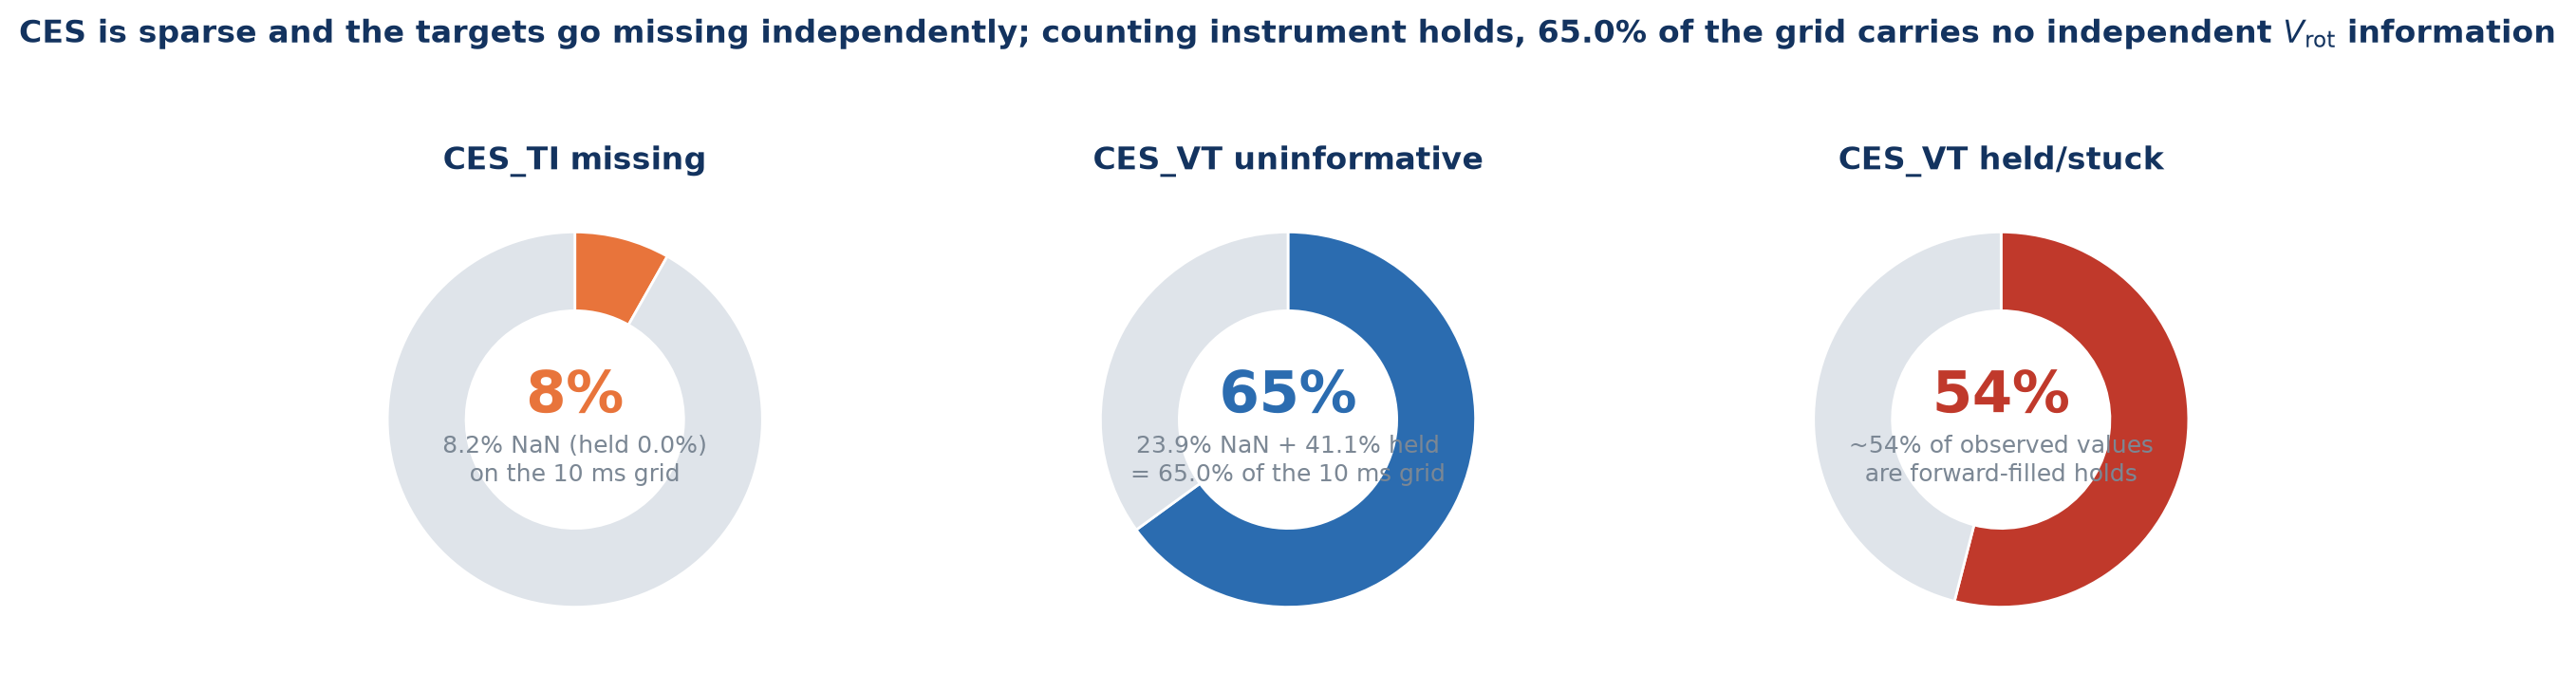
\includegraphics[width=0.72\linewidth]{fig_missing}
  \caption{10\,ms 격자에서의 CES 결측 구조. \Ti{}와 \Vrot{}은 독립적으로
  결측되며(8.2\% / 23.9\%), 행 필터링이 아닌 타겟별 마스킹을 요구한다. 계측기
  유지값까지 세면 격자의 65.0\%가 독립적인 \Vrot{} 정보를 갖지 않는다.}
  \label{fig:missing}
\end{figure}

\subsection{학습 예제의 두 가지 프레이밍}
\label{sec:framing}
\emph{윈도} 프레이밍(우리의 대조군, \S\ref{sec:model})은 타겟 인덱스 $t$의 샘플을
직전 $W$개 격자 행으로 구성한다: \texttt{bes} $(W,9)$,
\texttt{ecei} $(W,4)$, \texttt{mc} $(W,2)$, \texttt{time\_features} $(W,4)$,
\texttt{ces\_history} $(W,4)$, 정규화 타겟 $[\Ti,\Vrot]\in\mathbb{R}^2$,
그리고 타겟별 관측 마스크 $m\in\{0,1\}^2$. 네 개의 시간 특징---lookback
초, 행간 delta 초, 그리고 각각의 $\log(1{+}x)$ 변환---은 불규칙 관측 패턴을
명시적으로 노출한다(과거 CES 값의 신뢰도는 그것이 10\,ms 전 값인지 200\,ms 전
값인지에 강하게 의존한다). CES 이력의 네 채널은 직전 정규화 \Ti{}, 직전 정규화
\Vrot{}, 그리고 타겟마다 하나씩의 관측 플래그다. 본문 전체에서
$W{=}2$이다(\S\ref{sec:window}).

\emph{전체격자 시퀀스} 프레이밍(우리의 주 모델)은 고속 진단에 결측이 없다는
점을 이용해, 연속 세그먼트의 입력이 완전한 모든 행을---라벨 유무와
무관하게---맥락으로 유지한다. 각 스텝은 엄격히 인과적인 22개 채널을 담는다:
z-score된 15개 고속 채널, $\log(1{+}\Delta t_{\mathrm{prev}})$, 그리고 타겟별로
$t$ 이전 행에서 이월된 마지막 관측값, $\log(1{+}\text{경과시간})$, 과거 관측
존재 여부 플래그. 타겟은 병렬 관측 마스크와 함께 z-score되며, 희소성은 전적으로
손실에서 처리된다. 두 프레이밍 어느 쪽도 모델이 타겟 행 자신의 값을 읽게 하지
않는다.

\subsection{설계 원칙}
\begin{description}
  \item[가짜 라벨 금지.] 학습 행을 만들기 위해 타겟을 대체(impute)하지 않는다.
  윈도 프레이밍에서 행은 진단 입력이 완전하고 CES 타겟 중 \emph{적어도 하나}가
  실제로 관측된 경우에만 유지되며, 시퀀스 프레이밍에서 라벨 없는 행은 맥락으로만
  기여한다.
  \item[타겟별 마스킹 손실.] 손실은 타겟별로 마스킹된다:
  $\mathcal{L} = \sum_{k\in\{\Ti,\Vrot\}} m_k\,(\hat{y}_k-y_k)^2 / \sum_k m_k$.
  한 타겟만 관측된 행도 그 타겟은 학습에 기여한다. 두-타겟-필수 필터는 라벨 행의
  $\approx$28\%를 조용히 버렸을 것이며, 이를 제거한 것은 순수한 데이터 이득이다.
  \item[누수 방지.] (i) \emph{파일 단위 분할}: 한 shot 내 인접 행은 강하게
  자기상관되므로 분할은 shot 파일 단위로 이루어지고 디스크에 고정된다;
  (ii) \emph{학습 파일 전용 정규화}: 모든 $z$-score 통계(희소 타겟은
  NaN-인지)는 학습 파일에서만 추정되며, 시퀀스 모델은 여기에 더해 각 방전의
  고속 진단을 \emph{그 방전 자신의} 평균·분산으로 표준화한다---다른 방전도
  타겟도 사용하지 않는다(왜 중요한지는 \S\ref{sec:campaign});
  (iii) \emph{타겟 시점 마스킹}: 타겟 행 자신의 값과 관측 플래그는 입력에 결코
  들어가지 않는다.
\end{description}

\subsection{데이터 품질 감사 1: 유지(forward-fill)된 \Vrot{} 값}
\label{sec:stuck}
\textbf{관측된 \Vrot{} 값의 54\%가 계측기 유지값이다}: 같은 연속 시간 블록 안에서
직전 관측과 비트 단위로 동일한 반복(최대 1{,}214행 연속; 641개 중 499개 파일
영향)이다. \Vrot{}의 고유 측정 주기가 행 주기보다 느려 생기는 현상으로,
독립적인 측정이 아니다. \Vrot{}은 소수점 다섯 자리까지 기록되고 서로 다른 값
사이의 최소 간격이 $4\times10^{-5}$이므로 ``연속 동일''에는 측정 가능한 위양성
통로가 없으며, \Ti{}는 영향이 없다(226{,}991행 중 1행). 확정된 프로토콜에서
유지값은 \emph{모든 곳에서} 제거된다---지도 타겟, 이력·이월 입력과 그 관측
플래그, 정규화 통계, 그리고 모든 기준선의 보간 앵커에서---따라서 어떤 팔도
forward-fill로 공짜 점수를 받을 수 없다. 본 논문의 모든 수치는 진짜 측정만을
사용한다. 프로젝트 기록에는 이전의 유지값 포함 규약과, 유지값이 \emph{학습}도
오염시킴을 보인 짝지은 재학습(forward-fill 계단은 이력을 복사하는 것이 거의
최적이라고 모델에 가르친다)이 남아 있으며, 이것이 유지값 제거를 민감도 한 줄이
아니라 프로토콜로 삼은 이유다.

\subsection{데이터 품질 감사 2: \Ti{} 스펙트럼 피팅 실패와 두 모집단}
\label{sec:spikes}
관측된 \Ti{}의 p99는 $2{,}089$\,eV, p99.9는 $9{,}601$\,eV이고 최댓값은
14{,}984\,eV다. 이 먼 꼬리는 플라즈마 물리가 아니라 실패한 스펙트럼 피팅이다.
\textbf{1{,}197행(0.53\%)이 3\,keV를 초과}하며 274개 방전에서 951개의 런을
이룬다. 런의 85\%는 단일 행이고 5행 이상 지속하는 것은 2\%뿐이며, 런 정점의
중앙값은 관측된 이웃 평균의 13$\times$다(IQR 6--26$\times$). 이런 행은 어떤
방법으로도 예측 불가능하며, 공정한 비교에는 더 나쁘게도 \emph{보간 앵커로 쓰인}
스파이크가 그 이웃에서 보간을 오염시킨다. 두 가지 대응이 모두 방어 가능하고
각각 비판의 여지가 있다: $>$3\,keV를 모든 팔에서 결측으로 처리하면 어떤 방법도
예측할 수 없는 행을 제거하지만 ``어려운 행을 없앴다''는 비판을 부르고, 그대로
두면 스파이크 앵커를 먹인 채 오프라인 기준선에 핸디캡을 준다. 그래서 우리는
\textbf{두 개의 공동 1차 모집단}을 사전등록했다: \emph{컷}($>$3\,keV 값을 적재
시점에 결측으로 처리하며, 지도·이력 입력·정규화 통계·모든 기준선의 앵커에
동일하게 적용)과 \emph{포함}(컷 없음). \textbf{어떤 주장은 두 모집단 모두에서
성립할 때만 조건 없이 진술한다}. 한쪽에서만 성립하는 결과는 모집단을 명시해
보고한다. 임계값은 2.5--4\,keV 범위에서 무의미하다(\S\ref{sec:cutsens}). 값
기준 컷은 CES 피팅 품질 메타데이터가 확보되기 전까지 쓰는, 물리적으로 동기가
있는 대리 지표(``3\,keV 초과는 KSTAR 이온온도가 아니다'')이며 한쪽 방향뿐이다
---같은 감사는 어떤 값 컷도 건드리지 못하는 단일 표본 \emph{하향}
급락(양쪽 이웃의 $\tfrac12$ 이하인 4{,}965행)을 함께 찾아내고, 컷이 제거하는
것은 $\geq 2\times$ 상향 이상치의 19\%뿐이다. \Vrot{}에도 피팅 실패 스파이크가
있으나(16개 shot에서 1{,}000\,km/s를 넘는 119행, 그중 101행은 한 방전의 한
블록), 프로토콜은 \Vrot{}을 컷하지 않고 persistence 기반 \Vrot{} 비교마다 그
행들이 담는 제곱오차 비중을 보고한다.

% =========================================================================
\section{모델}
\label{sec:model}

주 모델 \seqv{}는 \textbf{357{,}570 파라미터}의 인과 시퀀스 나우캐스터이며,
그것이 대체한 윈도 모델은 201{,}258 파라미터의 후기 융합 네트워크로 짝지은
대조군으로 유지된다. 이 절은 그 두 모델을 기술하기 전에 \emph{무엇을 추정하는가},
\emph{왜 그 입력이 그 타겟에 배선되는가}, \emph{어떤 시간 척도 위에서 동작하는가}를
먼저 정한다. 셋 다 뒤의 결과 절이 측정한 양이 아니라 그 측정을 해석 가능하게
만드는 전제이며, 라우팅에 관해서는 설계 선택이 아니라 보존식의 결과다.

\subsection{추정 대상, 손실, 그리고 환원 불가능한 하한}
\label{sec:model:target}

모델은 각 격자 시각 $t$에서 정규화된 타겟 $y_t=[\Ti,\Vrot]_t$를 그 시각까지의
관측 이력 $x_{\le t}$로부터 추정한다. 손실은 타겟별 관측 마스크
$m_{t,c}\in\{0,1\}$ 위의 마스킹 평균제곱오차이며, 여기에 정규화 영점
$z_0$ 아래의 \Ti{} 예측을 억제하는 물리 페널티가 더해진다:
%
\begin{equation}
  \mathcal{L}
  = \frac{\sum_{t}\sum_{c\in\{\Ti,\Vrot\}} m_{t,c}\,\bigl(\hat y_{t,c}-y_{t,c}\bigr)^2}
         {\sum_{t}\sum_{c} m_{t,c}}
  \;+\; \lambda\,\overline{\mathrm{ReLU}\bigl(z_0-\hat y_{t,\Ti}\bigr)},
  \qquad \lambda = 0.1 .
  \label{eq:loss}
\end{equation}
%
식~\eqref{eq:loss}의 첫 항을 최소화하는 추정량은 조건부 기댓값
$\mathbb{E}[y_t\mid x_{\le t}]$이므로, 본 연구가 보고하는 것은 조건부 분포의
평균이지 그 분포 전체가 아니다. 불확실성은 별도로, 모델을 건드리지 않는 분포
무가정 구간으로 다룬다(\S\ref{sec:deploy}).

이 목표에는 추정기가 제거할 수 없는 하한이 있다. 타겟은 광자 적분 스펙트럼
피팅의 산물이므로 스스로 측정 잡음 $\sigma_\mathrm{meas}$를 지니며, 참 물리량을
완벽히 맞히는 예측자라도
%
\begin{equation}
  \mathrm{RMSE}^2 \;=\; \sigma_\mathrm{meas}^2 \;+\; b^2
  \label{eq:floor}
\end{equation}
%
를 기록한다($b$는 물리적 오차). 관측 계열 자체에서 차분 기반 추정기로 잰
$\sigma_\mathrm{meas}$는 컷 모집단 \Ti{}에서 \textbf{46.4--129.9\,eV}이다(4차
차분 상한 129.9, 상위 5\% 절사 68.7, 강건 MAD 46.4). 백본의 RMSE 157.8\,eV는
이 범위와 같은 자릿수이며, 두 끝값이 3배 가까이 벌어지는 이유가 손실의 성격을
결정한다: \textbf{4차 차분 제곱질량의 46.6\%(\Vrot{}은 65.6\%)가 상위 1\%의
한 스텝 변화에 몰려 있다.} 따라서 식~\eqref{eq:loss}의 총합은 \emph{꼬리
통계}이고, 폭과 계열이 평평하다는 뒤의 결과(\S\ref{sec:ladder})는 정보의 고갈이
아니라 이 사실의 귀결로 읽어야 한다. 본류에서는 모델이 여전히 타겟 자체 산포의
2.3--3.4배 위에 있다.

$\lambda=0.1$은 본 연구가 유도한 값이 아니라 윈도 파이프라인에서 물려받은
설정이며, 이를 유도로 바꾸는 방법은 위반율 목표를 정하고 승수를 제약 최적화로
푸는 것이다. 현재 판본은 그 대신 페널티가 결과를 만들지 않는다는 사실만
보고한다: 사다리의 모든 팔이 동일한 $\lambda$로 학습되며, 해석 가능한 칸
\bthree{}는 persistence에서 출발하는 구성상 페널티가 거의 활성화되지 않는데도
백본과 동급이다(\S\ref{sec:ladder}).

\subsection{두 보존식이 입력 라우팅을 정한다}
\label{sec:model:physics}

\seqv{}의 \Vrot{} 분기는 고속 진단을 보지 않는다. 이는 모델링 취향이 아니라
두 전송 방정식을 항별로 읽은 결과다. 이온 에너지와 토로이달 각운동량은
%
\begin{align}
  \frac{\partial}{\partial t}\Bigl(\tfrac{3}{2}n_i T_i\Bigr) + \nabla\!\cdot\!\mathbf{q}_i
    &= Q_{ei}\,(T_e-T_i) + S_i,
  \label{eq:energy}\\[2pt]
  \frac{\partial}{\partial t}\bigl(n_i m_i \langle R^2\rangle \omega_\varphi\bigr)
    + \nabla\!\cdot\!\Pi_\varphi
    &= T_\mathrm{NBI} + T_\mathrm{NTV} + T_\mathrm{int} + \cdots
  \label{eq:momentum}
\end{align}
%
를 따르며, 두 식 모두 \emph{값}이 아니라 \emph{변화율}을 구속한다. 그러므로
회전에 대해 물어야 할 것은 고속 진단이 \Vrot{}과 상관되는가가 아니라
$d\Vrot/dt$와 상관되는가이다. 식~\eqref{eq:momentum}의 각 항을 우리가 보유한
채널에 대조하면 표~\ref{tab:torque}가 된다.

\begin{table}[t]
  \centering
  \caption{식~\eqref{eq:momentum}의 항별 감사. 641개 방전 전수, 확정 데이터
  처리(스파이크 컷 후 유지값 제거), 624개 연속 블록. $r$은 모달리티 표준화 평균과
  타겟(또는 그 한 스텝 증분) 사이의 lag 0 통합 Pearson 상관이다.}
  \label{tab:torque}
  \small
  \begin{tabular}{llll}
    \toprule
    항 & 물리 & 우리 데이터에 있는가 & 판정 \\
    \midrule
    $\partial L/\partial t$ & 회전 변화율 & 연속 관측쌍의 차분 & 측정됨 \\
    $T_\mathrm{NBI}$ & 빔 토크 & 0-D 채널이 존재하지 않음 & 부재(\S\ref{sec:asym}) \\
    $T_\mathrm{NTV}\sim\delta B^2$ & 비축대칭 제동 & Mirnov, 100\,Hz 데시메이트 & 음성 종결 \\
    $\nabla\!\cdot\!\Pi_\varphi$ & 난류 운동량 유속 & BES가 밀도요동을 봄 & \textbf{측정 $\rightarrow$ 널} \\
    $T_\mathrm{int}$ & 잔여응력 & $\nabla T_i$ 필요, 스칼라만 보유 & 도달 불가 \\
    \bottomrule
  \end{tabular}
\end{table}

$T_\mathrm{NTV}$는 이미 닫힌 항이다: Mirnov는 100\,Hz로 데시메이트되어
$|\mathrm{MC}|$와 이동 RMS 같은 진폭 대리 지표가 모두 도움이 되지 않았다
(\S\ref{sec:asym}). 남아 있던 유일한 항은 난류 운동량 유속이며, BES가 그것이
올라타는 밀도요동을 보므로 원리상 도달 가능하다. 측정 결과는 널이다:
%
\[
  \underbrace{r\bigl(\mathrm{BES},\,d\Vrot/dt\bigr) = -0.006,\qquad
              r\bigl(\mathrm{ECEI},\,d\Vrot/dt\bigr) = -0.003}_{\text{운동량식}}
  \qquad\text{대}\qquad
  \underbrace{+0.070,\qquad +0.078}_{\text{에너지식}(d\Ti/dt)}
\]
%
값 수준에서도 같은 비대칭이 나타난다(BES$\rightarrow$\Ti{} $+0.341$,
ECEI$\rightarrow$\Ti{} $+0.311$ 대 \Vrot{} $+0.027$, $+0.005$). \emph{같은
측정이 에너지식에서는 신호를 잡으므로 회전의 널은 방법의 한계가 아니다.}
$T_\mathrm{NBI}$가 데이터셋에 없고 $T_\mathrm{NTV}$가 닫혔으며
$T_\mathrm{int}$가 도달 불가인 상태에서 마지막 항까지 널이므로, 우리 입력이
식~\eqref{eq:momentum}을 통해 \Vrot{}에 닿을 경로는 남아 있지 않다. 인코더에서
분기를 나누는 설계는 이 감사의 구현이며, 그 결과 15개 고속 채널을 전부 교란해도
\Vrot{} 출력이 비트 단위로 동일하다(\S\ref{sec:asym}). 남은 레버는 모델이 아니라
취득이다(\S\ref{sec:headroom}).

\subsection{모델이 놓인 시간 척도}
\label{sec:model:scales}

세 개의 시간이 이 문제를 규정한다. 첫째, 격자 간격 $\Delta t = 10$\,ms이므로
Nyquist 주파수는
%
\begin{equation}
  f_\mathrm{Nyq} = \frac{1}{2\,\Delta t} = 50~\mathrm{Hz}
  \label{eq:nyquist}
\end{equation}
%
이다. Mirnov가 담아야 할 모드 회전은 kHz 대역이고(본 데이터셋의 방전들에서
보고된 EHO 조화파는 약 4와 8\,kHz이다), 반앨리어싱 필터 없이 100\,Hz로
데시메이트된 $dB/dt$는 표본화 정리상 그것을 표현할 수 없다. \S\ref{sec:asym}의
lag-1 자기상관 $-0.009$(BES $+0.568$ 대비)는 이 사실의 \emph{확인}이지 그
근거가 아니다.

둘째, 전자와 이온을 결합시키는 시간이다. Braginskii 전자 충돌시간
$\tau_e = 3.44\times10^{5}\,T_e^{3/2}/(Z\,n_e\ln\Lambda)$(초, $T_e$는 eV,
$n_e$는 cm$^{-3}$)로부터 온도 평형화 시간은
%
\begin{equation}
  \tau_\mathrm{eq} \simeq \frac{m_i}{2m_e}\,\tau_e
  \label{eq:taueq}
\end{equation}
%
이다. 중수소, $\ln\Lambda=17$, $Z=1$에서 $\tau_\mathrm{eq}$는 $T_e=0.5$--3\,keV와
$n_e=2$--$5\times10^{19}$\,m$^{-3}$ 범위에서 8.3--305\,ms이고, 관측된 \Ti{}
중앙값 593\,eV에 대응하는 구석에서는 \textbf{8--59\,ms}이다. 본 연구가 측정한
연속 인과 문맥의 포화점은 약 50\,ms이며, 두 수는 같은 자릿수다. 이는
자릿수 수준의 정합성 진술이고 그 이상이 아니다: 식~\eqref{eq:taueq}의 플라즈마
파라미터는 인용값이며(BES와 ECEI는 계측기 단위이므로 본 연구는 $n_e$와 $T_e$를
물리 단위로 갖지 않는다) 앞의 상수에는 order-unity 관례가 있다.

셋째, 신호가 스스로를 닮아 있는 시간이다. 641개 파일에서 잰 자기상관의 $1/e$
시간은 \Ti{} 159\,ms, BES 161\,ms, ECEI 147\,ms로 서로 10\% 이내에서 일치한다.
\Vrot{}은 그렇지 않다: 관측의 54\%가 계측기 유지값이므로 유지값을 제거하면
16\,ms, 유지하면 300\,ms를 넘어 19배 이상 벌어진다. \textbf{\Vrot{}의 완화
시간은 이 데이터셋에서 측정 불가능하다.} \Ti{}는 641개 파일에서 유지값이 1행뿐이라
이 문제를 겪지 않는다. 유지값 병리는 값의 54\%뿐 아니라 그 물리량의 동역학을
특징지을 능력까지 앗아간 것이며, 이는 NBI 토크와 원본 kHz Mirnov에 이은 세 번째
취득 과제다(\S\ref{sec:headroom}). 이 자기상관들은 추세를 제거하지 않고 계산되어
방전 포락선이 지배하므로 수송 시간 $\tau_E$나 $\tau_\varphi$로 인용하지 않는다.

\subsection{전체격자 인과 시퀀스 백본}
\label{sec:model:backbone}

\seqv{}는 세그먼트의 22채널 격자 시퀀스(\S\ref{sec:framing}) 위에서 서로 독립인
두 개의 인과 LSTM을 돌린다. \Ti{} 분기(2층, 160 유닛)는 전체 상태---고속 진단,
두 타겟의 이월값, 경과시간 플래그, $\Delta t$---를 읽고, \Vrot{} 분기(1층,
64 유닛)는 \emph{고속이 아닌 7개 채널만} 읽는다: $\Delta t$와 타겟별 이월값,
경과시간, 관측 플래그. 이 배선이 \S\ref{sec:model:physics}의 항별 감사를 그대로
구현한 것이다. 각 분기는 LayerNorm과 작은 GELU 헤드로 끝나며, 출력은
행별 정규화 $[\Ti, \Vrot]$이고 손실은 식~\eqref{eq:loss}를 세그먼트의 모든 라벨
행에 대해 적용한 것이다. 이 프레이밍에서 두 가지가 따라 나온다. 첫째, 모델이
과거로 뻗는 \emph{도달 범위}가 고정 윈도가 아니라 세그먼트 전체다---\S\ref{sec:gate}에서 이
모델을 모든 윈도 변형과 가르는 바로 그 양이다. 둘째, 라우팅이 \emph{인코더}
수준에서 성립한다: 순환 상태를 공유하면 헤드를 어떻게 배선하든 고속 진단 정보가
\Vrot{} 헤드로 흘러들지만, 여기서는 15개 고속 채널을 전부 교란해도 \Vrot{}
출력이 비트 단위로 동일하다(\S\ref{sec:asym}).

\subsection{윈도 대조군: 관측 마스킹 어텐션 풀링}
\label{sec:model:window}

대조군은 각 모달리티(BES, ECEI, MC)를 $W{=}2$ 윈도 위의 전용 시간 인지 1-D
CNN으로 인코딩하고, CES 이력을 양방향 GRU(은닉 64)로 읽은 뒤 시점별 출력을
타겟마다 하나씩 두 개의 독립적인 멀티헤드 가산 어텐션 readout으로 풀링하되,
\emph{하드 마스킹}하여 어텐션 질량이 \emph{그} 타겟이 실제로 측정된 행에만
놓이도록 한다---보간 자신의 귀납 편향(관측된 표본만 사용)을 파라미터 비용 0으로
어텐션에 써 넣은 것이다. \Ti{} 헤드는 고속 진단·시간·이력을 융합하고, \Vrot{}
헤드는 이력과 시간만 융합한다. 두 모델이 공유하는 모든 것---데이터 계약, 유지값
제거 처리, 타겟별 마스킹, 분할, 채점 모집단---은 동일하게 고정되므로 두 모델의
비교는 행 단위로 짝지어진다.

\subsection{해석 가능한 사다리 칸}
\label{sec:model:rung}

\bthree{}(\S\ref{sec:ladder})는 \seqv{}의 프레이밍과 라우팅을 유지하되 각 헤드를
\emph{정확한} 분해로 대체한다: $\hat y = \text{이월값} +
\sum_k w_k z_k + b$, 여기서 $z\in[-1,1]^K$는 작은 인과 GRU(64/32 유닛, \Ti{}는
$K{=}8$, \Vrot{}은 4)의 tanh 잠재이고 readout은 0으로 초기화되어 학습이 정확히
persistence에서 시작한다. 파라미터는 21{,}498개로 백본의 6\%다.

\subsection{최적화 설정, 그리고 그 근거의 현황}
\label{sec:model:optim}

학습은 AdamW($\eta=10^{-3}$, weight decay $10^{-4}$), 배치 16 세그먼트,
gradient norm clipping 1.0, 검증 마스킹 MSE에 대한 \texttt{ReduceLROnPlateau}
(patience 2, factor 0.5)와 조기 종료(patience 6, 최대 30 epoch; 확정 실행은
14--25 epoch에서 멈췄다)를 사용한다.

이 값들은 \emph{유도된 것이 아니라} 윈도 파이프라인에서 물려받은 것이며, 본
연구는 그 사실을 감추지 않는다. 데이터와 구조의 축은 전부 통제 실험으로 닫혔지만
(윈도 크기 \S\ref{sec:window}, 유지값 처리 \S\ref{sec:stuck}, 두 모집단
\S\ref{sec:spikes}, 복잡도와 폭 \S\ref{sec:ladder}), 최적화 축은 그런 측정을
거치지 않았다. 현재 이 설정을 방어하는 증거는 하나뿐이며 그것은 간접적이다:
백본 관문의 \emph{예산 균등화} 조건은 두 모델을 고정 10 epoch로 학습시키고 검증
기반 체크포인트 선택을 금지하는데, 그 조건에서도 백본의 짝지은 \Ti{} 이득은
4개 분할 전부 양수였다($+0.063$, $+0.033$, $+0.045$, $+0.030$;
\S\ref{sec:selection}). 즉 결론은 학습 일정의 인공물이 아니다.

그럼에도 ``왜 배치 16인가''에는 아직 답이 없고, 음성이나 공백은 그것을 뒤집을
측정을 함께 지목해야 한다는 본 연구의 규칙(\S\ref{sec:headroom})이 여기에도
적용된다. 두 가지가 이 공백을 닫는다. 첫째, 경사 잡음 척도(gradient noise scale)를
한 번 측정하면 이 문제의 임계 배치가 정해지고 배치 16이 그 아래인지 위인지가
선택이 아니라 결과가 된다. 둘째, 폭에 따라 최적 학습률이 이동하지 않는
파라미터화($\mu$P)를 쓰면 \S\ref{sec:ladder}의 폭 스윕이 평평한 이유가 ``용량이
도움이 되지 않는다''인지 ``학습률이 그 폭에 맞지 않았다''인지의 구분이 구성상
불필요해진다. 둘 다 재학습 규모가 작고 test를 건드리지 않는다.

\paragraph{탐색이 가르쳐 준 것.}
윈도 계열에 대한 두 라운드의 통제된 아키텍처 반복에서(선택은 깨끗한 검증
skill만으로), 살아남은 메커니즘은 어텐션 풀링 하나뿐이었고 용량 확장·스킵
위상·추가 추출기는 한 번도 도움이 되지 않았다. 확정된 프로토콜 아래에서 같은
교훈이 두 번 더 반복된다: \seqv{}에 관측 마스킹 인과 어텐션을 더한 것은 작고
일관되게 양수이지만 유의하지 않은 이득이었고(\S\ref{sec:selection}), \seqv{}의
5점 폭 스윕은 평평하다(\S\ref{sec:ladder}). 이 문제의 병목은 용량이 아니라
정보이며, 식~\eqref{eq:floor}와 표~\ref{tab:torque}가 그 병목이 각각 어디에
있는지를 타겟별로 말해 준다.

% =========================================================================
\section{평가 방법론}
\label{sec:eval}

\paragraph{지표.}
모든 오차는 물리 CES 단위로 역정규화되어 타겟별로 계산된다. 1차 점수는
사전등록된 헤드라인 기준선에 대한 Murphy skill~\citep{murphy1988},
$\skillp = 1 - \mathrm{MSE}_{\mathrm{model}}/\mathrm{MSE}_{\mathrm{PCHIP}}$
(양수 = 모델 우위; 0 = 동률)이다. 모든 팔(모델과 모든 기준선)은 \emph{동일한}
(파일, 행) 샘플 집합에서 동일한 타겟별 유지 마스크로 채점되며, 어떤 짝지은 비교
이전에도 모집단 키가 비트 단위로 동일함을 검증한다. 보간은 타겟 자신의 값을
제외한다(누수 없음). 보간도 모델 입력도 세그먼트 경계를 넘지 않으며, 경계 너머의
이웃이 필요한 지점에서는 보간이 persistence 값을 대신 예측한다(모집단 축소
없음, PR2).

\paragraph{기준선 사다리.}
persistence와 국소 과거 전용 AR은 최초 사전등록의 인과 기준이고, 선형·PCHIP·
가우시안 과정(정확한 Matérn-3/2 + 백색잡음, 최근접 16+16 국소 적합, 표본별
주변우도 격자 선택, PR2 fallback을 그대로 상속)은 미래를 읽는다. 인과 쪽에는
\textbf{인과 GP}를 추가한다: 같은 GP를 과거 이웃 16개로 제한하고 NaN 조건을
동일하게 두어 채점 모집단이 움직이지 않게 한 것이다. 이것이 배치 가능한 가장
강한 기준선임은 분명하며(시드 42 \Ti{} RMSE 164.3 대 persistence 197.2, 컷
모집단), ``배치 가능한 모든 인과 방법을 이긴다''는 persistence가 아니라 이
기준선에 대해 판정한다.

\paragraph{3분할; 선택은 TEST를 보지 않는다.}
파일들은 train/val/test로 분할된다. 모든 분할의 test 파일은 어떤 아키텍처 탐색
\emph{이전에} 예약되었고 모델 선택 과정에서 절대 읽지 않는다. 표준(시드 42)
test 셋은 컷 모집단에서 96개 shot에 걸친 관측 \Ti{} $n = 32{,}589$행과 60개
shot에 걸친 진짜 \Vrot{} $n = 10{,}463$행을 담는다(포함 모집단은
$32{,}721$ / $10{,}461$). 4개 분할(시드 42, 1, 7, 123)은 각각 96개 shot에 걸쳐
\Ti{} 32.6--35.9k행, 60--66개 shot에 걸쳐 \Vrot{} 10.5--14.5k행을 담는다. 본
논문의 모든 수치는 단일 수집 스크립트가 동결된 실행 디렉터리에서 읽어오므로,
본문·표·그림이 서로 어긋날 수 없다.

\paragraph{사전등록.}
해당 test 수치를 보기 전에 문서로 고정한 규칙들은 다음과 같다.
\textbf{PR1} 헤드라인 비교 대상은 PCHIP(과도 현상에서의 단조성·무진동을 근거로
사전 선택; 사다리 전체도 함께 보고);
\textbf{PR2} 보간은 모델이 채점되는 모든 곳에서 예측하며, 미래 이웃이 없으면
persistence로 후퇴하고 그 후퇴 비율을 보고한다(채점된 \Ti{} 행의 0.3--0.4\%,
그러나 \textbf{채점된 \Vrot{} 행의 40--44\%}이므로 \Vrot{}의 ``PCHIP 대비''는
5분의 2가 ``persistence 대비''다);
\textbf{PR3} test 셋 최소 규모($\geq$15 shot, $\geq$3{,}000 관측 \Ti{} 샘플;
전부 충족);
\textbf{PR4} 유의성은 skill에 대한 shot 군집 bootstrap 95\% CI가 0을 제외하는
것으로 정의. 확정된 프로토콜은 여기에 다음을 더한다: 유지값 제거 학습·채점;
24-run 스윕의 plateau 최소 규칙에 따른 $W{=}2$(\S\ref{sec:window}); 윈도 계열의
파일당 샘플 상한 500; \S\ref{sec:spikes}의 두 공동 1차 모집단; 그리고 백본
관문, 단 하나의 어텐션 후보, 해석 가능한 사다리 칸, 폭 스윕에 대해
\emph{TEST 채점 이전에 확정한 모델 결정 규칙}(\S\ref{sec:selection}). 임계값
민감도(2.5/3/4\,keV)도 보고한다.

\paragraph{Shot 군집 paired bootstrap.}
한 방전 내 인접 CES 행은 강하게 상관된다. 샘플을 독립으로 취급하면 불확실성이
크게 과소평가된다. 샘플별 짝지은 오차
$\mathrm{SE}_{\mathrm{model}}-\mathrm{SE}_{\mathrm{PCHIP}}$를 shot 단위로
집계하고, shot 전체를 복원추출로 재표본한다(10{,}000회, 고정 시드). 얻어진 CI는
진짜 shot 간 일반화를 반영한다. 대가는 유효 표본 크기가 shot 수(\Ti{}는
$\approx$96, \Vrot{}은 60--66)가 된다는 것이며, 이것이 전체 검정력을 제한한다.
모델 대 모델 비교(백본 대 대조군, 사다리 칸 대 백본)도 같은 행 위에서 같은
paired bootstrap을 사용한다.

\paragraph{MNAR 문제와 그에 대한 우리의 대응.}
진짜 결측 시점에는 참값이 없으므로 skill은 \emph{관측된} 시점을 가려 측정한다.
CES 결측은 MNAR이므로(저신호, ELM, 천이에서 탈락) 관측 시점 skill은 진짜 결측
시점 성능의 낙관적 추정이다. \S\ref{sec:mnar}에서 채점된 지점들을 \emph{실제로
결측인} 지점들의 공변량 분포 위로 재가중하여 skill이 얼마나 살아남는지를
보고하고, 아울러 결측 모집단 중 애초에 이 분석의 도메인 안에 있는 비율도 함께
보고한다.

% =========================================================================
\section{결과}
\label{sec:results}

\subsection{나우캐스터는 모든 인과 기준선을 압도한다}
표~\ref{tab:ladder}는 표준 test 분할에서의 물리 단위 RMSE 사다리를 보여준다.
\seqv{}는 미래를 읽지 않는 모든 방법 가운데 두 타겟 모두에서 최저 RMSE를 가지며,
배치 가능한 가장 강한 팔인 인과 GP를 RMSE 기준 4\%(\Ti{})와 18\%(\Vrot{}) 차로
이기고, 미래를 쓰는 보간들도 앞선다. 유일하게 동률인 팔은 잡음 앵커를 통과하는
대신 평균해 내는 오프라인 GP다(\Ti{} 153.8 대 157.8). 이는 본 논문에서 가장
강건한 결과다: 미래 CES가 정의상 없는 모든 온라인 환경에서 시퀀스 나우캐스터는
명백한 승자다.

\begin{table}[t]
  \centering
  \caption{물리 단위 RMSE 사다리. 표준 held-out test 분할(시드 42), 컷 모집단,
  진짜 측정만($n = 32{,}589$ \Ti{}, $10{,}463$ \Vrot{}). 낮을수록 좋다. 아래쪽
  세 행은 미래를 읽는다. 포함 모집단에서는 \seqv{} 363.0 / 23.7, PCHIP
  412.4 / 30.2, 인과 GP 394.6 / 28.8, persistence 478.0 / 33.4(\Ti{} / \Vrot{})로,
  피팅 실패 스파이크가 모든 \Ti{} RMSE를 두 배 이상으로 키우지만 순서는 바꾸지
  않는다.}
  \label{tab:ladder}
  \small
  \begin{tabular}{llrr}
    \toprule
    팔 & 정보 접근 & \Ti{} RMSE (eV) & \Vrot{} RMSE (km/s) \\
    \midrule
    \textbf{\seqv{} (나우캐스터)} & 고속 진단 + 과거 CES, 세그먼트 전체 & \textbf{157.8} & \textbf{23.6} \\
    윈도 대조군 ($W{=}2$) & 고속 진단 + 과거 CES 2행 & 169.2 & 26.1 \\
    인과 GP & 과거 CES 이웃 16개 & 164.3 & 28.8 \\
    Persistence & 마지막 관측 CES & 197.2 & 33.4 \\
    AR (국소, 인과) & 과거 CES만 & 472.2 & 51.0 \\
    \midrule
    GP (오프라인) & 과거 + 미래 CES & 153.8 & 24.7 \\
    선형 보간 & 과거 + 미래 CES & 169.8 & 29.0 \\
    PCHIP 보간 & 과거 + 미래 CES & 173.6 & 30.2 \\
    \bottomrule
  \end{tabular}
\end{table}

\begin{figure}[t]
  \centering
  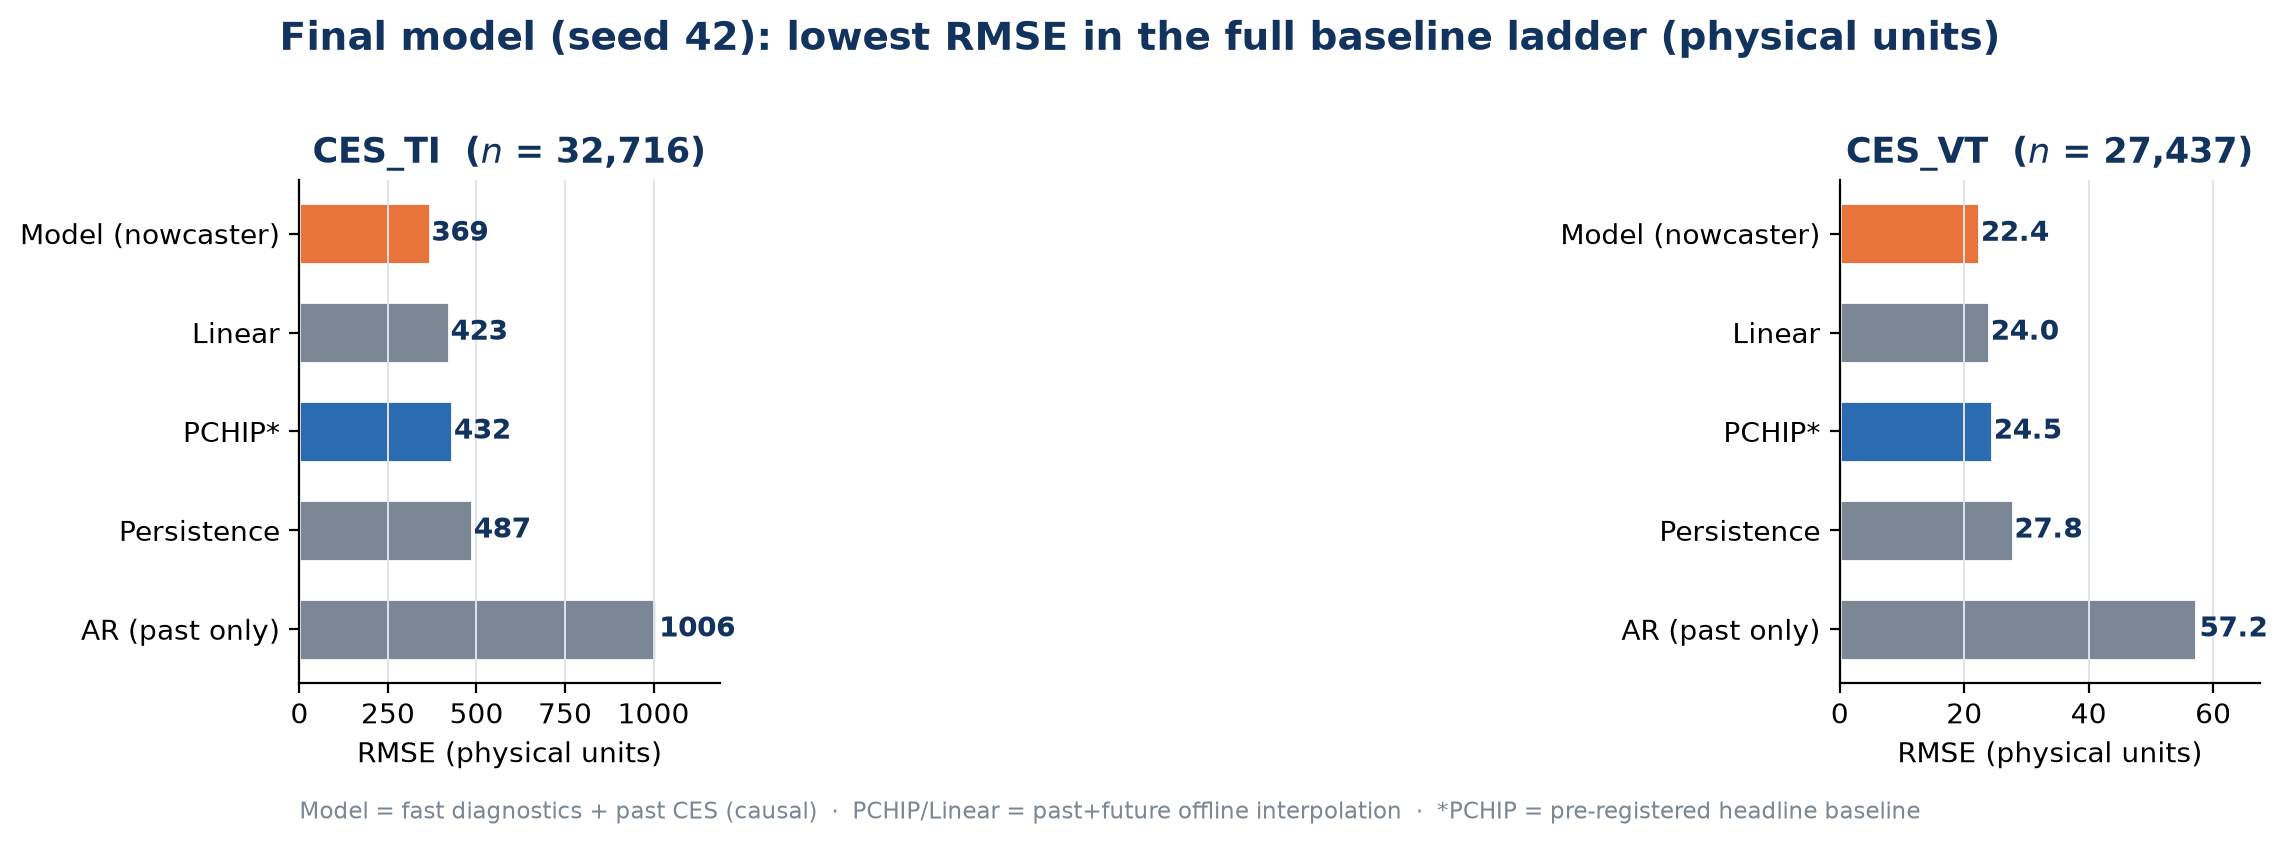
\includegraphics[width=0.9\linewidth]{fig_rmse_ladder}
  \caption{시드 42 test 분할의 RMSE 사다리(컷 모집단, 진짜 측정): 인과
  나우캐스터가 두 타겟 모두에서 배치 가능한 방법 중 최저 RMSE를 달성하고 미래를
  쓰는 보간도 앞선다. 표~\ref{tab:ladder}와 같은 수치이며, 둘 다 같은 동결
  산출물에서 생성된다.}
  \label{fig:ladder}
\end{figure}

\subsection{헤드라인: \Ti{}는 두 모집단 모두에서 4개 독립 분할에 걸쳐 미래를 쓰는
보간을 이긴다}
\label{sec:headline}
표~\ref{tab:headline}은 두 공동 1차 모집단에서 4개 독립 held-out 분할(시드 42,
1, 7, 123 --- 뒤의 셋은 어떤 선택 단계에도 쓰이지 않았다)에 대한 백본의 성능을
PCHIP 대비와 인과 GP 대비로 보고한다. 그림~\ref{fig:forest}는 PCHIP 대비
신뢰구간을 보여준다.

\begin{table}[t]
  \centering
  \caption{\seqv{}의 held-out test $\skillp$와 shot 군집 95\% CI(10{,}000회
  재표본), 두 모집단. 마지막 열은 같은 행 위에서 인과 GP에 대해 짝지은 skill이다.
  굵은 글씨 = PASS(CI가 0을 제외).}
  \label{tab:headline}
  \small
  \begin{tabular}{llccc}
    \toprule
    타겟 & 분할 & 컷: $\skillp$ (95\% CI) & 포함: $\skillp$ (95\% CI) & 인과 GP 대비 (컷 / 포함) \\
    \midrule
    \multirow{4}{*}{\Ti{}}
      & 42  & $\mathbf{+0.174}$ $[+0.097, +0.236]$ & $\mathbf{+0.225}$ $[+0.109, +0.293]$ & $\mathbf{+0.078}$ / $\mathbf{+0.154}$ \\
      & 1   & $\mathbf{+0.248}$ $[+0.188, +0.295]$ & $\mathbf{+0.238}$ $[+0.153, +0.302]$ & $\mathbf{+0.133}$ / $\mathbf{+0.169}$ \\
      & 7   & $\mathbf{+0.257}$ $[+0.199, +0.302]$ & $\mathbf{+0.292}$ $[+0.232, +0.344]$ & $\mathbf{+0.138}$ / $\mathbf{+0.123}$ \\
      & 123 & $\mathbf{+0.264}$ $[+0.188, +0.320]$ & $\mathbf{+0.316}$ $[+0.186, +0.392]$ & $\mathbf{+0.105}$ / $\mathbf{+0.149}$ \\
    \midrule
    \multirow{4}{*}{\Vrot{}}
      & 42  & $\mathbf{+0.390}$ $[+0.077, +0.591]$ & $\mathbf{+0.384}$ $[+0.066, +0.586]$ & $\mathbf{+0.331}$ / $\mathbf{+0.324}$ \\
      & 1   & $+0.183$ $[-0.028, +0.280]$ & $\mathbf{+0.195}$ $[+0.000, +0.286]$ & $+0.130$ / $\mathbf{+0.143}$ \\
      & 7   & $+0.135$ $[-0.358, +0.269]$ & $+0.132$ $[-0.362, +0.266]$ & $+0.020$ / $+0.018$ \\
      & 123 & $+0.305$ $[-0.049, +0.437]$ & $+0.304$ $[-0.065, +0.433]$ & $\mathbf{+0.134}$ / $+0.132$ \\
    \bottomrule
  \end{tabular}
\end{table}

\begin{itemize}
  \item \textbf{\Ti{}: 두 모집단 모두에서 4개 분할 전부 PASS.}
        $\skillp$는 컷에서 $+0.17\sim+0.26$, 포함에서 $+0.23\sim+0.32$이며 모든
        shot 군집 CI가 0을 제외한다. 8개 모집단--분할 셀 전부가 \emph{인과}
        GP($+0.08\sim+0.17$)와 persistence($+0.36\sim+0.46$)도 이긴다. 이것이
        본 논문의 무조건적 주장이다. 오프라인 GP를 상대로는 백본이
        \emph{동률}이므로(점추정 $-0.05\sim+0.11$, 8개 중 1개 셀에서 유의),
        관측 모집단에 대한 주장은 ``사전등록된 보간들과 배치 가능한 모든 인과
        방법을 이기고, 미래를 쓰며 표본별로 튜닝된 평활기와는 대등하다''로
        읽힌다.
  \item \textbf{\Vrot{}: 승리가 아니라 동률.} 두 모집단 모두에서 점추정은 모든
        분할에서 양수지만, PR4를 통과하는 것은 1/4(컷)과 2/4(포함)이다---둘 다
        시드 42, 그리고 포함 모집단의 시드 1이 $[+0.000, +0.286]$이다.
        persistence 대비로는 두 모집단 모두 3/4 분할에서
        통과하고($+0.30\sim+0.50$; 시드 7의 CI는 0에 닿는다) 인과 GP 대비로는
        2/4다. 4개 중 1--2개 유의는 잡음이 만들어낼 수 있는 수준이므로 회전
        채널의 승리는 주장하지 않는다.
  \item \textbf{왜 포함 모집단의 수치가 더 높은가.} 컷이 없으면 모든 팔이 PCHIP을
        상대로 \emph{더 좋은} 점수를 받는다(백본 평균 $+0.268$ 대 $+0.236$,
        대조군 $+0.238$ 대 $+0.173$). 스파이크가 보간 앵커를 오염시키기
        때문이다: 학습된 모델은 스파이크가 낀 이월값을 할인할 수 있지만 보간은
        그럴 수 없다. \S\ref{sec:asym}이 이 성분을 정량화하며, 이것이 어느 한
        모집단만 인용하지 않는 이유다.
\end{itemize}

\begin{figure}[t]
  \centering
  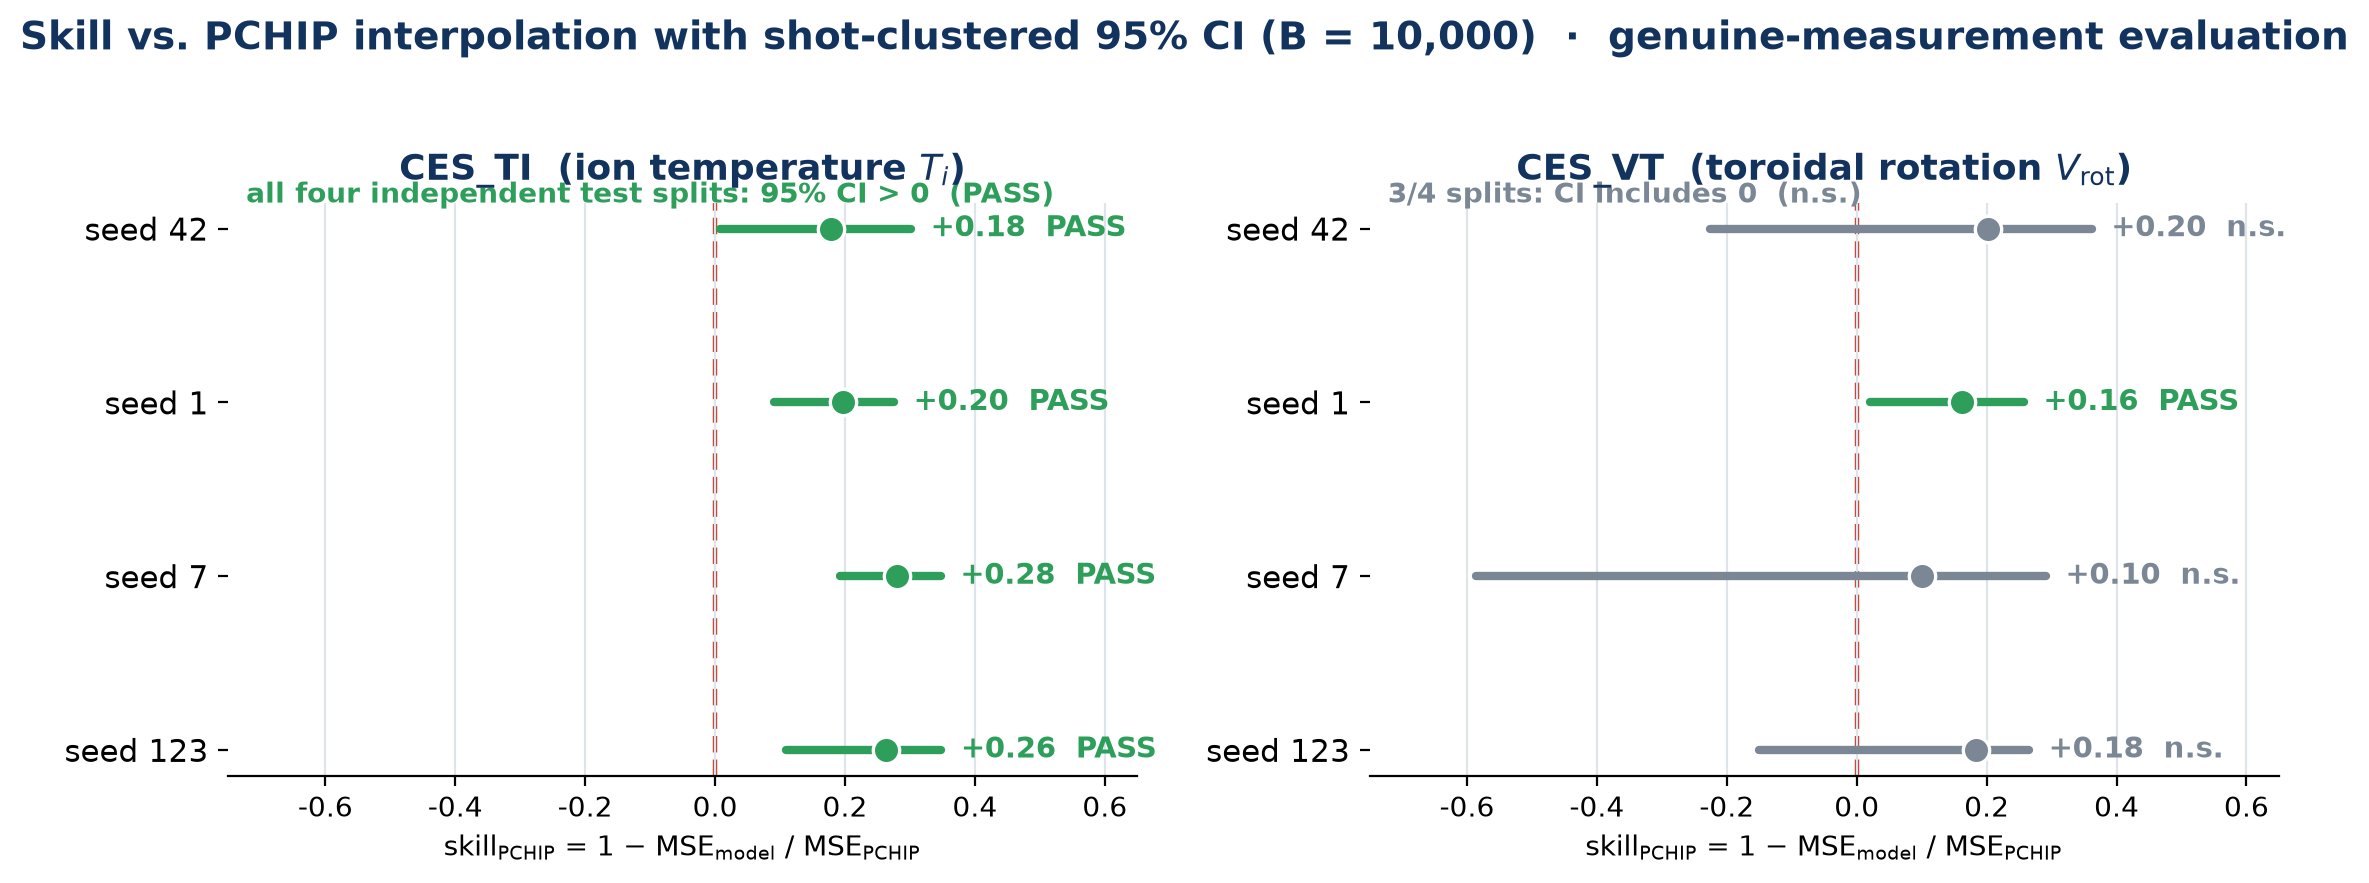
\includegraphics[width=0.92\linewidth]{fig_forest}
  \caption{두 모집단, 4개 독립 held-out 분할에 걸친 \seqv{}의 $\skillp$와 shot
  군집 95\% CI의 forest plot. \Ti{}는 8개 셀 전부에서, \Vrot{}은 3개 셀에서 0을
  제외한다.}
  \label{fig:forest}
\end{figure}

\subsection{전체격자 프레이밍 대 윈도 대조군: 백본 관문}
\label{sec:gate}
시퀀스 프레이밍을 채택할 만했는가? 이 결정은 네 개의 조건을 갖춘 관문으로
사전등록되었고 한 번만 채점되었다(컷 모집단 --- 내부 모델 선택이 수행되는
모집단이다): 분할 시드 $\times$ 초기화 시드의 $4\times 4$ 격자를 돌리고, 각
실행을 해당 분할의 $W{=}2$ 윈도 대조군과 행 단위로 짝지었다. 짝지은 \Ti{}
skill은 \textbf{16/16 실행에서 양수였고 13/16에서 개별적으로 유의}했다. 분할별
초기화 평균은 $+0.129$, $+0.059$, $+0.078$, $+0.058$이고(초기화 산포가 분할
산포보다 훨씬 작다), 통합 평균은 실행 군집 95\% CI $[+0.067, +0.096]$과 함께
$\mathbf{+0.081}$이다. 예산을 균등화한 팔(고정 10 epoch, 최종 가중치, 검증 선택
없음)도 4/4 분할에서 부호를 유지하므로($+0.063$, $+0.033$, $+0.045$, $+0.030$)
이 이득은 학습 예산 효과가 아니라 아키텍처에서 온다. 그리고 어떤 실행도 유의한
\Vrot{} 손실을 보이지 않았다(8/16은 유의한 승리). 네 조건이 모두 성립했다. 본
논문의 나머지 전부에서 보고되는 4개 확정 분할에서 같은 비교는 컷에서 $+0.130$,
$+0.058$, $+0.062$, $+0.044$, 포함에서 $+0.053$, $+0.024$, $+0.047$, $+0.029$로
8/8 양수이고 각 모집단에서 2/4 유의다.

이 관문은 프레이밍이 \emph{무엇을} 사는지도 확정한다. 윈도 대조군은 인과 GP와
동률인 반면(컷 기준 1/4 분할 유의) 시퀀스 백본은 두 모집단 모두에서 4/4로
이긴다: 세그먼트의 과거 전체로 뻗는 도달 범위가 배치 가능한 가장 강한 기준선을
넘어서게 하는 요소다. 그 비용은 음수다---샘플별 윈도 조립도 조합적 증강도 없기
때문에 백본은 윈도 계열의 학습 시간 중 일부만으로 학습된다.

\subsection{skill이 사는 곳: 간극 영역}
\label{sec:gap}
마지막 관측 CES로부터의 경과시간 $\Delta t$로 계층화하면, 채점 타겟의
$\geq$96\%가 인접 영역($\Delta t \leq 15$\,ms)에 있다. 분할별로는 넓은 구간에
수백 개 샘플밖에 없으므로 \emph{4개 test 분할을 통합}하고 bootstrap을 물리적
방전 단위로 군집한다(표~\ref{tab:gap}). $\Delta t$가 커질수록 PCHIP의 과제는
\emph{쉬워지고}(간극을 사이에 둔 두 실제 관측을 보간한다) 우리 과제는 어려워지므로,
이 영역은 인과 방법이 이길 것으로 기대하기 가장 어려운 곳이다.

\begin{table}[t]
  \centering
  \caption{간극 계층별 skill. 4개 test 분할 통합, shot 군집 95\% CI, \seqv{}.
  굵은 글씨 = CI가 0을 제외. 샘플이 50개 미만인 행은 채점하지 않는다.}
  \label{tab:gap}
  \small
  \begin{tabular}{lrrcc}
    \toprule
    $\Delta t$ & $n$ (컷 / 포함) & shot 수 & 컷: PCHIP 대비 & 포함: PCHIP 대비 \\
    \midrule
    \multicolumn{5}{l}{\emph{\Ti{}}}\\
    $\leq 15$\,ms & 134{,}546 / 135{,}317 & 301 & $\mathbf{+0.239}$ $[+0.197, +0.274]$ & $\mathbf{+0.299}$ $[+0.244, +0.347]$ \\
    $> 15$\,ms    &   3{,}422 /   3{,}334 & 265 / 263 & $\mathbf{+0.268}$ $[+0.187, +0.337]$ & $\mathbf{+0.206}$ $[+0.108, +0.290]$ \\
    $> 45$\,ms    &      460 /      429 & 104 / 101 & $\mathbf{+0.267}$ $[+0.092, +0.414]$ & $-0.004$ $[-0.304, +0.246]$ \\
    \midrule
    \multicolumn{5}{l}{\emph{\Vrot{}}}\\
    $\leq 15$\,ms & 51{,}689 & 197 & $\mathbf{+0.233}$ $[+0.020, +0.318]$ & $\mathbf{+0.233}$ $[+0.020, +0.317]$ \\
    $> 15$\,ms    &      466 / 456 & 130 & $\mathbf{+0.418}$ $[+0.104, +0.680]$ & $\mathbf{+0.432}$ $[+0.128, +0.696]$ \\
    $> 45$\,ms    &       14 & 7 & --- & --- \\
    \bottomrule
  \end{tabular}
\end{table}

\paragraph{\Ti{}의 승리는 인접 이력에 국한되지 않는다.} 15\,ms를 넘어서도 백본은
두 모집단 모두에서 미래를 쓰는 PCHIP을 이기고($+0.268$과 $+0.206$, 두 CI 모두 0
위), 거기서 persistence는 $+0.40$과 $+0.43$으로 이긴다. 45\,ms를 넘어서면 컷에서는
여전히 이기지만($+0.267$) 포함 모집단에서는 \emph{동률}이다($-0.004$, CI
$[-0.30, +0.25]$): 101개 shot의 429행은 소수의 스파이크 앵커 행이 한 계층을
지배할 수 있는 바로 그 지점이며, 우리는 이를 동률로 보고한다.

\paragraph{\Vrot{}은 보간에게 가장 어려운 그 한 곳에서 보간을 이긴다.} 전역
\Vrot{} 동률은 인접 영역에서의 동률이다. $\Delta t > 15$\,ms에서는 백본이 두
모집단 모두에서 PCHIP을 이기며($+0.418$과 $+0.432$, 130개 shot) --- 본 논문에서
유일한 무조건적 \Vrot{} 긍정 판정이다 --- $\leq 15$\,ms에서는 persistence를
이긴다($+0.39$). 가장 넓은 구간은 14행뿐이라 채점하지 않는다.

\subsection{실제로 결측인 지점에서는 이 중 얼마가 살아남는가?}
\label{sec:mnar}

지금까지의 모든 것은 마침 \emph{관측된} CES 지점에서 측정된 것이다. 참값이 없는
곳에서 오차를 측정할 수는 없다. 그러나 관측 행과 결측 행 \emph{모두}에서 계산
가능한 공변량 위에서 skill이 어떻게 변하는지는 측정할 수 있고, 재가중할 수 있다.
기전을 담는 공변량은 둘이다: 마지막 진짜 관측으로부터의 $\Delta t$(15/25/45\,ms로
구간화)와 \S\ref{sec:peak}의 입력 전용 국소 활동 플래그다. 후자는 자기 행을
제외한 이웃 집합으로 계산되므로 결측 행에서도 정의된다. $\Delta t \times$ 활동으로
사후 계층화하고, 채점 샘플이 30개 미만인 계층은 버리며, 모든 추정치 옆에 살아남은
커버리지를 함께 보고한다. 가중 격자는 모집단과 일관되게 만든다(컷은 여기에도
적용한다). 한 계층 안에서 결측 행과 관측 행이 교환 가능하다는 가정은 없앤 척하지
않고 명시한다.

\paragraph{먼저, 적용 범위에 관한 결과.} 이 분석의 도메인은 ``해당 타겟의 진짜
관측이 두 행 이내에 있음''이라는 $W{=}2$ 기준이다. 진짜 결측인 \Ti{} 행 가운데
분할별로 \textbf{54--68\%가 도메인 안}이고, 진짜 결측인 \Vrot{} 행 가운데는
\textbf{4--6\%뿐}이다. \Vrot{} 간극이 긴 블록이기 때문이다(살아남은 계층의
커버리지는 \Ti{} 0.99, \Vrot{} 0.73--0.76). 따라서 재가중된 \Vrot{} 행은 결측
질량의 20분의 1에 대한 질문에 답하는 것이며, 우리는 거기서 아무것도 끌어내지
않는다.

\begin{table}[t]
  \centering
  \caption{관측 모집단에서 진짜 결측이면서 도메인 안인 모집단으로 재가중한
  \seqv{}의 \Ti{} skill(계층 가중치를 고정한 shot 군집 95\% CI). 굵은 글씨 =
  CI가 0을 제외. \emph{무가중}은 표~\ref{tab:headline}의 헤드라인이다.}
  \label{tab:mnar}
  \small
  \begin{tabular}{llcccc}
    \toprule
    & & \multicolumn{2}{c}{PCHIP 대비} & \multicolumn{2}{c}{persistence 대비} \\
    \cmidrule(lr){3-4}\cmidrule(lr){5-6}
    모집단 & 분할 & 무가중 & 결측 정합 (95\% CI) & 무가중 & 결측 정합 (95\% CI) \\
    \midrule
    \multirow{4}{*}{컷}
      & 42  & $+0.174$ & $+0.140$ $[-0.071, +0.290]$ & $+0.360$ & $\mathbf{+0.398}$ $[+0.278, +0.518]$ \\
      & 1   & $+0.248$ & $\mathbf{+0.164}$ $[+0.062, +0.250]$ & $+0.406$ & $\mathbf{+0.366}$ $[+0.299, +0.448]$ \\
      & 7   & $+0.257$ & $+0.203$ $[-0.024, +0.346]$ & $+0.403$ & $\mathbf{+0.310}$ $[+0.227, +0.398]$ \\
      & 123 & $+0.264$ & $\mathbf{+0.283}$ $[+0.069, +0.392]$ & $+0.415$ & $\mathbf{+0.381}$ $[+0.246, +0.464]$ \\
    \midrule
    \multirow{4}{*}{포함}
      & 42  & $+0.225$ & $\mathbf{+0.140}$ $[+0.033, +0.250]$ & $+0.423$ & $\mathbf{+0.443}$ $[+0.141, +0.623]$ \\
      & 1   & $+0.238$ & $\mathbf{+0.217}$ $[+0.086, +0.319]$ & $+0.436$ & $\mathbf{+0.383}$ $[+0.273, +0.536]$ \\
      & 7   & $+0.292$ & $\mathbf{+0.167}$ $[+0.067, +0.265]$ & $+0.406$ & $\mathbf{+0.283}$ $[+0.172, +0.380]$ \\
      & 123 & $+0.316$ & $\mathbf{+0.221}$ $[+0.050, +0.320]$ & $+0.459$ & $\mathbf{+0.337}$ $[+0.164, +0.455]$ \\
    \bottomrule
  \end{tabular}
\end{table}

\paragraph{둘째, 두 비교가 갈라지며 --- 그 갈라짐 자체가 쓸모 있는 것이다.}
\textbf{persistence --- 온라인 시스템이 실제로 돌리는 기준선 --- 를 상대로는 \Ti{}
우위가 두 모집단 모두에서 4개 분할 전부 재가중을 견딘다}($+0.28\sim+0.44$, 모든
CI가 0을 제외). MNAR 보정이 앗아가는 skill은 많아야 $0.12$이고 어떤 분할에서는
전혀 없다. \textbf{미래를 쓰는 PCHIP}을 상대로는 재가중된 점추정이
$+0.14\sim+0.28$에 머물지만, 고정 가중치의 넓은 CI가 컷 모집단 2개 분할에서 0을
지난다(2/4 유의; 포함 모집단은 4/4). 결측 지점은 더 큰 $\Delta t$에 놓이는데,
그곳이 바로 양쪽 앵커가 가장 크게 도움이 되고 재가중 bootstrap이 가장 얇은
곳이다. 따라서 정말 중요한 지점들에서 증거가 지지하는 주장은 다음과 같다:
\emph{진짜 결측이면서 도메인 안인 시점에서 나우캐스터는 두 모집단 모두에서 CES
단독의 어떤 인과 방법보다 유의하게 낫고, 오프라인 보간보다는 모집단 조건부
유의성(컷 2/4, 포함 4/4)으로 낫다}. 윈도 대조군도 같은 방식으로 거동한다
(PCHIP 대비 2/4와 4/4, persistence 대비 4/4).

\subsection{캠페인 이동을 견디는가?}
\label{sec:campaign}

무작위 분할이 하지 않지만 실제 배치가 하는 두 번째 일은 시간상 앞으로 나아가는
것이다. 641개 방전 전부를 shot 번호(30801--32751)로 정렬하고 시간으로 엄격히
잘랐다: \textbf{train 416 shot [30801, 31991], val 128 [32002, 32310], test 97
[32312, 32751]}이며 어떤 test shot도 어떤 train shot보다 앞서지 않는다. 나머지는
전부 헤드라인 프로토콜에 고정되어 바뀐 변수는 분할 규칙 하나뿐이다. 분할이
고정되어 있으므로 네 번의 실행은 \emph{초기화} 시드만 달리하며, 이를 4개 분할인
것처럼 제시하지 않고 그대로 밝힌다. 모집단마다 세 개의 팔을 둔다: 헤드라인에서
학습된 그대로의 윈도 대조군(학습 파일 전용 정규화), 고속 진단을 shot별로
표준화한 같은 대조군(컷 모집단), 그리고 \seqv{}이다(표~\ref{tab:campaign},
그림~\ref{fig:campaign}).

\begin{table}[t]
  \centering
  \caption{시간(캠페인) 분할, 4개 초기화, 뒤쪽 방전 97개로 이루어진 TEST 블록.
  항목은 $\skillp$이며 \textbf{굵은 글씨} = PR4 PASS. 마지막 열은 같은 행 위에서
  윈도 대조군에 대한 \seqv{}의 짝지은 \Ti{} skill이다.}
  \label{tab:campaign}
  \small
  \resizebox{\linewidth}{!}{%
  \begin{tabular}{llcccc}
    \toprule
    모집단 & 팔 & \Ti{} PCHIP 대비 (초기화 42 / 1 / 7 / 123) & PASS & \Ti{} 인과 GP 대비 & \seqv{} $-$ 대조군 \\
    \midrule
    \multirow{3}{*}{컷}
      & 윈도 대조군 (OFF) & $+0.027$ / $\mathbf{+0.091}$ / $-0.001$ / $\mathbf{+0.061}$ & 2/4 & 0/4 & --- \\
      & 대조군, shot별 표준화 (ON) & $\mathbf{+0.103}$ / $\mathbf{+0.107}$ / $\mathbf{+0.094}$ / $\mathbf{+0.107}$ & 4/4 & --- & --- \\
      & \seqv{} & $\mathbf{+0.187}$ / $\mathbf{+0.174}$ / $\mathbf{+0.181}$ / $\mathbf{+0.177}$ & 4/4 & 4/4 ($+0.11\sim+0.12$) & $\mathbf{+0.164}$ / $\mathbf{+0.091}$ / $\mathbf{+0.182}$ / $\mathbf{+0.124}$ \\
    \midrule
    \multirow{2}{*}{포함}
      & 윈도 대조군 (OFF) & $+0.014$ / $+0.047$ / $+0.055$ / $+0.089$ & 0/4 & 0/4 & --- \\
      & \seqv{} & $\mathbf{+0.173}$ / $\mathbf{+0.202}$ / $\mathbf{+0.198}$ / $\mathbf{+0.184}$ & 4/4 & 4/4 ($+0.13\sim+0.16$) & $\mathbf{+0.161}$ / $\mathbf{+0.163}$ / $\mathbf{+0.151}$ / $\mathbf{+0.104}$ \\
    \bottomrule
  \end{tabular}}
\end{table}

\begin{figure}[t]
  \centering
  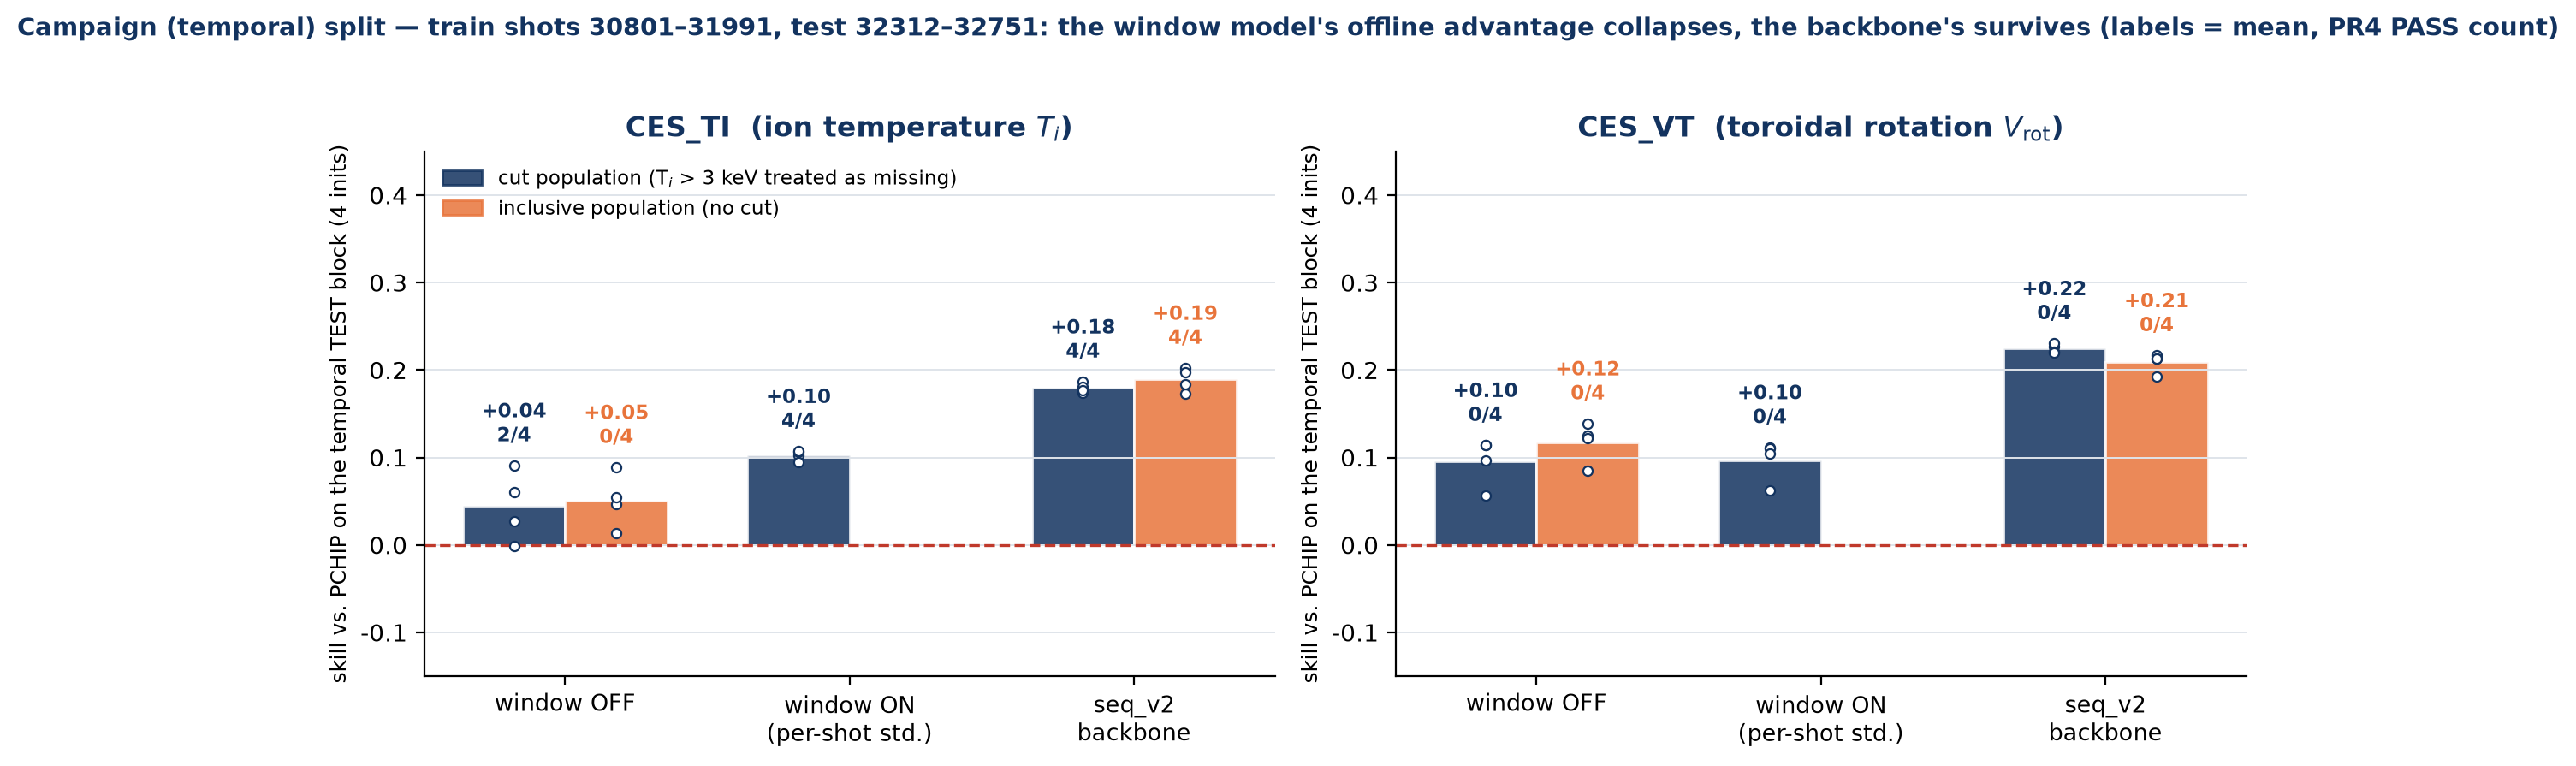
\includegraphics[width=0.92\linewidth]{fig_campaign}
  \caption{캠페인(시간) 분할: 윈도 대조군의 보간 대비 우위는 붕괴하고, shot별
  표준화가 이를 복구하며, 시퀀스 나우캐스터는 두 모집단 모두에서 우위를 유지한다.
  막대는 4개 초기화의 평균이며 초기화별 점과 PR4 카운트를 함께 표시한다.}
  \label{fig:campaign}
\end{figure}

이 표에서 명시할 만한 것이 셋 있다. 첫째, \emph{윈도} 모델의 오프라인 보간 대비
우위는 이동을 견디지 못한다: 2/4(컷)와 0/4(포함) 초기화이며, 인과 GP 대비로는
0/4다. 둘째, 이름이 지목되었던 그 수리가 작동한다: 각 방전의 고속 진단을
\emph{그 방전 자신의} 평균·분산으로 적재 시점에 표준화하면(타겟은 손대지 않는다)
컷 모집단의 관문이 2/4에서 4/4로 올라가고 짝지은 값은 $+0.078$, $+0.018$,
$+0.095$, $+0.049$(3/4 유의)이며 \Vrot{}은 변하지 않는다($-0.003\sim+0.008$)
---\Vrot{} 헤드가 고속 진단을 애초에 보지 않으므로 기대되는 음성 대조다. 셋째,
그리고 이것이 이 절의 결과다: \textbf{시퀀스 나우캐스터는 붕괴하지 않는다}. 두
모집단 모두에서 4/4 초기화에 대해 PCHIP을 이기고($+0.17\sim+0.20$), 두 모집단
모두에서 4/4로 인과 GP를 이기며($+0.11\sim+0.16$), 8/8에서 윈도 대조군을 이긴다.
\Vrot{}은 윈도 대조군이 0/4인 자리에서 두 모집단 모두 4/4로 persistence를
이기고($+0.31\sim+0.34$), 대조군 대비 \Vrot{} 마진은 8/8에서
유의하다($+0.06\sim+0.18$).

\paragraph{대조군이 왜 나빠지는가 --- 단언이 아니라 측정.}
전이에 실패해야 하는 것은 \emph{고속 진단} 경로다. CES 단독 보간 대비 우위를
사는 것이 바로 그 경로인 반면, CES 이력 경로는 두 기간 모두에서 같은 물리량을
같은 단위로 보기 때문이다. 대조군이 정규화된 그 단위에서 채널별
train$\rightarrow$test 드리프트를 측정하면 이것이 확인된다: 위치 이동의 중앙값은
\textbf{BES가 1.22\,$\sigma$}, \textbf{ECEI가 0.53\,$\sigma$}이고 척도 비는
각각 $0.75$와 $0.62$인 반면, \textbf{CES 타겟 자신은 0.115\,$\sigma$에 척도 비
$1.06$}이다. 고속 진단은 예측 대상보다 5--11$\times$ 더 이동한다. 학습 파일
전용 정규화(\S\ref{sec:data})는 무작위 분할에서는 올바른 누수 방지 선택이지만
캠페인 이동에서 바로 그것이 깨진다. shot별 표준화는 그 방전 자신의 데이터만
쓰므로 누수가 없다. \seqv{}는 정의상 shot별로 표준화하며---이것이 전이가 되는 두
이유 중 하나이고, 다른 하나는 도달 범위다(\S\ref{sec:gate}).

\paragraph{두 개의 스트레스 테스트, 하나의 독법.}
표~\ref{tab:stress}는 채택된 모델에 대해 둘을 나란히 놓는다. 실시간 시스템이
실제로 돌릴 수 있는 기준선들에 대한 우위는 두 모집단 모두에서 두 스트레스
테스트를 모두 견딘다. \emph{미래를 쓰는} 보간에 대한 우위는 두 모집단 모두에서
시간 이동을 견디고, MNAR 재가중은 모집단 조건부 유의성으로 견딘다. 이 표의 윈도
모델 판본---본 연구의 이전 초안이 보고했던 것---에서는 오프라인 우위가 두 테스트
\emph{모두} 견디지 못했다. 그것을 바꾼 것이 시퀀스 프레이밍이며, 새 열이 원래부터
거기 있었던 것처럼 제시하지 않고 그대로 밝힌다.

\begin{table}[t]
  \centering
  \caption{스트레스 하의 두 주장, \seqv{}, \Ti{}. 항목은 PR4 통과 수(컷 / 포함)와
  점추정 범위다.}
  \label{tab:stress}
  \small
  \resizebox{\linewidth}{!}{%
  \begin{tabular}{lcc}
    \toprule
    평가 & PCHIP 대비 (오프라인, 미래 사용) & 인과 기준선 대비 \\
    \midrule
    무작위 분할, 관측 지점 & \textbf{4/4 / 4/4}, $+0.17\sim+0.32$ & 인과 GP 대비 \textbf{4/4 / 4/4}, $+0.08\sim+0.17$ \\
    결측 지점으로 재가중 (\S\ref{sec:mnar}) & 2/4 / \textbf{4/4}, $+0.14\sim+0.28$ & persistence 대비 \textbf{4/4 / 4/4}, $+0.28\sim+0.44$ \\
    시간 캠페인 분할 (\S\ref{sec:campaign}) & \textbf{4/4 / 4/4}, $+0.17\sim+0.20$ & 인과 GP 대비 \textbf{4/4 / 4/4}, $+0.11\sim+0.16$ \\
    \bottomrule
  \end{tabular}}
\end{table}

\paragraph{남는 단서.} 네 번의 캠페인 통과는 하나의 시간 test 블록 위의
초기화들이므로 이는 4개 분할의 증거가 아니라 하나의 시간 분할의 증거이며, 컷
모집단 \seqv{} 캠페인 실행 4개 중 2개는 30-epoch 상한에서 멈췄다.

\subsection{\Ti$\leftrightarrow$\Vrot{} 정보 비대칭}
\label{sec:asym}
윈도 대조군에 대한 통제된 입력 모달리티 절제---한 모달리티 그룹을 \emph{평가
시점에} 0으로 만들고, 재학습은 하지 않으며, persistence와 보간은 실제 이력에서
계산---는 두 타겟이 왜 다르게 거동하는지를 설명하고 \S\ref{sec:model}의 라우팅을
확정된 프로토콜 아래에서 다시 근거 짓는다(표~\ref{tab:ablation},
그림~\ref{fig:ablation}).

\begin{table}[t]
  \centering
  \caption{$W{=}2$ 윈도 대조군의 평가 시점 모달리티 절제, TEST, 두 모집단:
  $\skillp$(4개 분할 평균)와 절제하지 않은 실행에 대한 짝지은 변화
  (분할 42 / 1 / 7 / 123; $^{*}$ = 유의하게 악화).}
  \label{tab:ablation}
  \small
  \resizebox{\linewidth}{!}{%
  \begin{tabular}{llcc}
    \toprule
    입력 & 타겟 & 컷 & 포함 \\
    \midrule
    전체 (이력 + 고속 + 시간) & \Ti{} & $+0.173$ & $+0.238$ \\
    이력 + 시간만 (\emph{고속 없음}) & \Ti{} & $-0.125$; 짝지은 $-0.25^{*}$ / $-0.38^{*}$ / $-0.42^{*}$ / $-0.43^{*}$ & $+0.201$; 짝지은 $-0.03^{*}$ / $-0.04$ / $-0.03$ / $-0.09^{*}$ \\
    고속 + 시간만 (\emph{이력 없음}) & \Ti{} & $-2.11$; 짝지은 $-4.6^{*}$ / $-1.8^{*}$ / $-2.3^{*}$ / $-1.9^{*}$ & $-1.16$; 짝지은 $-1.5^{*}$ / $-3.4^{*}$ / $-1.2^{*}$ / $-1.1^{*}$ \\
    \midrule
    전체 & \Vrot{} & $+0.213$ & $+0.206$ \\
    이력 + 시간만 (\emph{고속 없음}) & \Vrot{} & $+0.213$; 짝지은 $+0.000$ $\times 4$ (\textbf{비트 동일}) & $+0.206$; 짝지은 $+0.000$ $\times 4$ (\textbf{비트 동일}) \\
    고속 + 시간만 (\emph{이력 없음}) & \Vrot{} & $-2.89$; 짝지은 $-5.4^{*}$ / $-6.3^{*}$ / $-1.8^{*}$ / $-2.3^{*}$ & $-3.51$; 짝지은 $-6.9^{*}$ / $-7.8^{*}$ / $-1.9^{*}$ / $-2.2^{*}$ \\
    \bottomrule
  \end{tabular}}
\end{table}

\begin{figure}[t]
  \centering
  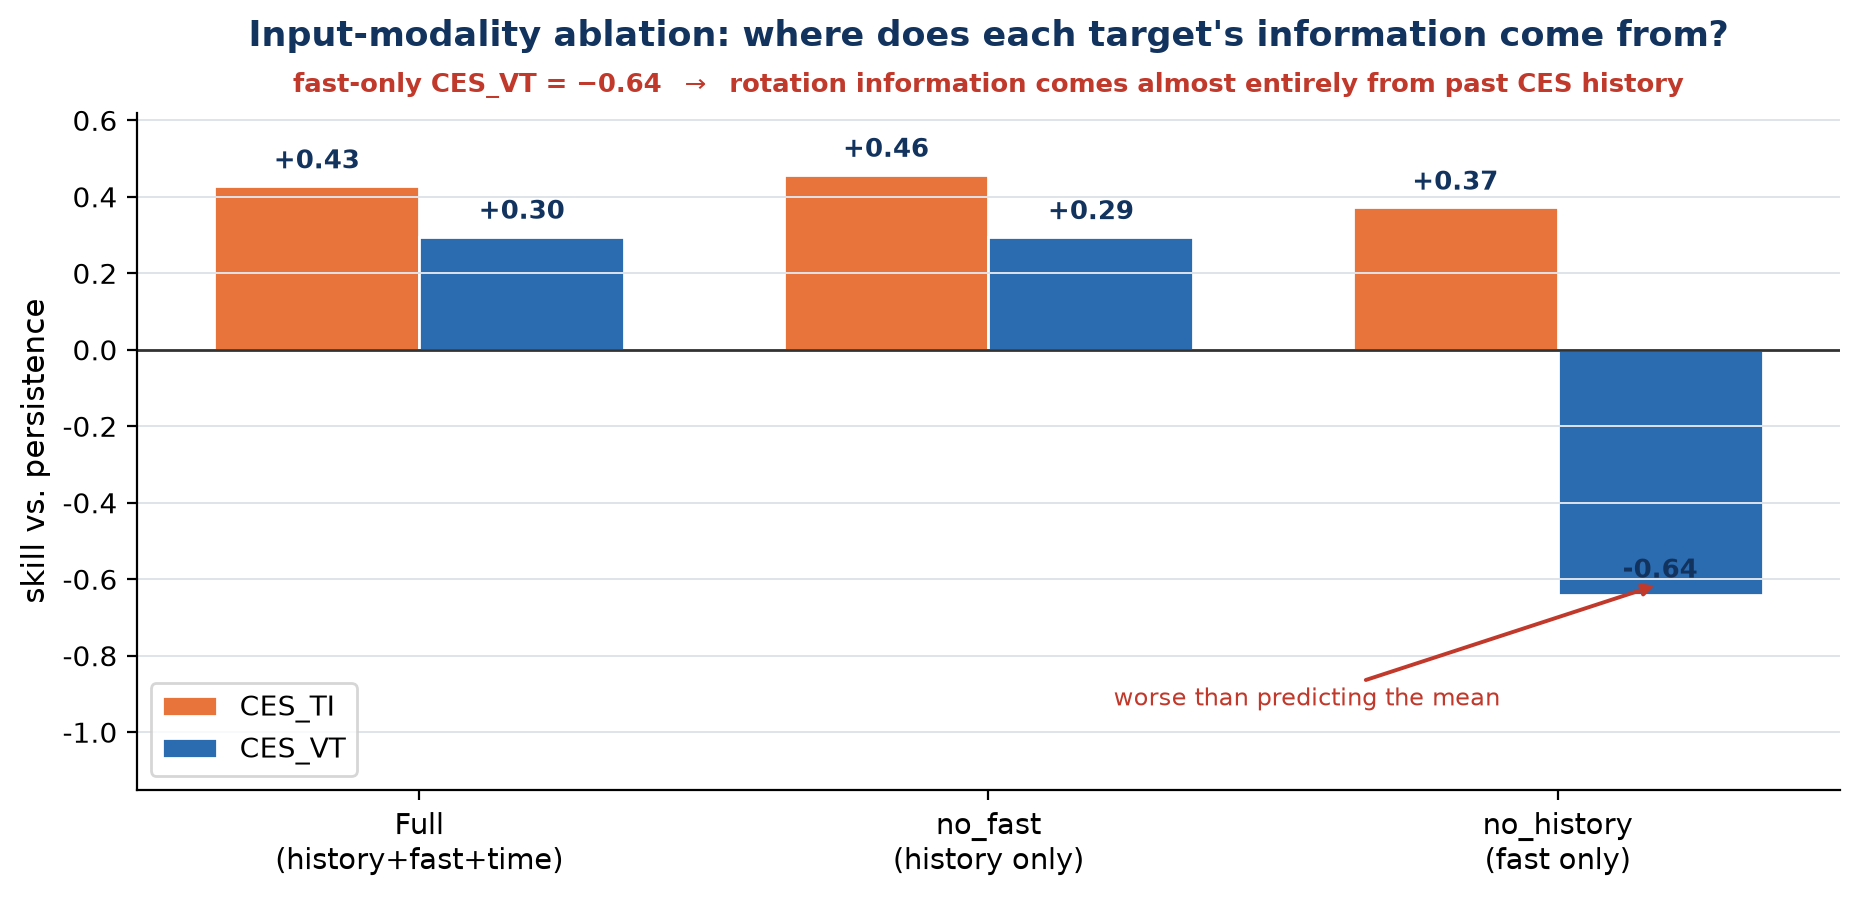
\includegraphics[width=0.92\linewidth]{fig_ablation}
  \caption{윈도 대조군의 평가 시점 모달리티 절제, 두 모집단. 고속 진단을 0으로
  만들면 \Vrot{}은 비트 단위로 동일하고 컷에서는 \Ti{} 마진이 사라진다. 이력을
  0으로 만들면 두 타겟 모두 붕괴한다.}
  \label{fig:ablation}
\end{figure}

\begin{itemize}
  \item \textbf{이력은 두 타겟 모두에 필수불가결하다.} CES 이력이 없으면 윈도
        모델은 두 모집단의 두 타겟 모두에서 PCHIP 대비 $-1$에서 $-4$까지
        떨어진다: 자기 앵커 없이 100\,Hz 진단만으로 예측 가능한 타겟은 없다.
  \item \textbf{\Ti{}: 보간 대비 마진은 고속 진단 정보다 --- 컷 모집단에서.}
        BES/ECEI/MC를 0으로 만들면 대조군은 보간기 \emph{아래로}
        떨어진다($-0.10\sim-0.18$; 짝지은 변화 $-0.25\sim-0.43$, 4/4 유의).
        물리 채널은 충돌성 전자--이온 결합이며($t_{ei}\propto T_e^{3/2}/n_e$),
        ECEI가 $T_e$를, BES가 $n_e$ 구조를 공급한다.
  \item \textbf{포함 모집단에서는 같은 이력 전용 모델이 여전히 PCHIP을
        $+0.15\sim+0.23$로 이기며}, 고속 채널이 더하는 것은 $0.03$--$0.09$뿐이다
        (2/4 유의). 보간기의 앵커에 스파이크가 끼어 있고, 학습된 모델은 보간이
        할 수 없는 방식으로 그것을 할인하기 때문이다. 따라서 스파이크 포함
        마진에는 고속 진단 정보가 아닌 \emph{스파이크 강건성} 성분이 들어 있으며,
        이것이 본 논문이 더 좋아 보이는 한쪽이 아니라 두 모집단을 보고하는 측정된
        이유다. 고속 진단의 기여를 분리해 내는 쪽은 컷 모집단이다.
  \item \textbf{\Vrot{}: 정보는 전적으로 CES 이력이며, 구조적으로도 측정으로도
        그렇다.} 고속 진단을 0으로 만들어도 \Vrot{} 출력은 8/8 모집단--분할
        셀에서 \emph{비트 단위로 동일}하고(라우팅이 구조적이다), \seqv{}와
        \bthree{}의 \Vrot{} 분기도 같은 교란 시험을 통과한다. 토로이달 회전은
        우리 입력 중 어느 것도 관측하지 않는 운동량 원천---외부 NBI 토크와 고유
        회전 구동~\citep{Rice2007IntermachineComparison}---이 지배하며, Mirnov
        신호는 100\,Hz로 샘플되어 회전의 대리가 될 수 있었을 kHz 모드 회전
        주파수를 앨리어싱으로 잃는다(\S\ref{sec:headroom}).
\end{itemize}

이 비대칭은 절제 실험 이전에 물리로부터 예측되었고 절제로 확인되었다. \Vrot{}의
비승리는 모델의 실패가 아니라 진단 정보량에 관한 발견이며, \S\ref{sec:model}의
타겟별 라우팅을 정당화한다.

\subsection{이력은 얼마나 필요한가? 관측 하나}
\label{sec:window}

윈도 계열의 이력 윈도는 원래 검토되지 않은 기본값이었다($W{=}4$). 우리는 그 단언을
곡선과 명시된 선택 규칙으로 대체했다: \textbf{24회의 독립 실행},
$W \in \{2,3,4,6,8\} \times$ 시드 $\{42,1,7,123\}$에 더해 \emph{history-0} 지점
$\times$ 4시드이며, 각각 헤드라인과 동일한 프로토콜(유지값 제거, 파일당 상한 500,
스파이크 컷 없음---이 스윕은 컷보다 앞서며, 동결된 $W{=}2$ 실행이
\S\ref{sec:headline}의 포함 모집단 대조군이다)로 자기 held-out test 분할에서
채점된다. 세 가지 통제가 지점들을 비교 가능하게 만든다: 파일 단위 분할이 윈도에
불변이고(모든 실행이 시드별로 같은 96개 test shot을 평가한다), 파일당 상한이
시간 부분집합 증강---$W{=}2$의 240k 샘플에서 $W{=}8$의 30.1M으로 폭발한다---이
소수의 긴 블록 방전에 지배되는 것을 막으며, 채점 모집단은 $W{=}2$에서 $W{=}8$까지
1.8\%만 줄어든다.

\begin{table}[t]
  \centering
  \caption{Window 스윕, 4시드에 걸친 held-out test $\skillp$ 평균(PASS = shot
  군집 95\% CI가 0을 제외하는 시드 수). History-0은 $W{=}4$에서의
  \texttt{no\_history} 절제이며, $W{=}1$은 구성할 수 없다.}
  \label{tab:window}
  \small
  \begin{tabular}{rrrcrc}
    \toprule
    이력 관측 수 & $W$ & \Ti{} skill & PASS & \Vrot{} skill & PASS \\
    \midrule
    0 & 4 & $-0.026$ & 0/4 & $-0.783$ & 0/4 \\
    1 & 2 & $+0.238$ & \textbf{4/4} & $\mathbf{+0.206}$ & 0/4 \\
    2 & 3 & $\mathbf{+0.246}$ & \textbf{4/4} & $+0.203$ & 1/4 \\
    3 & 4 \emph{(구 기본값)} & $+0.221$ & 3/4 & $+0.190$ & 1/4 \\
    5 & 6 & $+0.190$ & 3/4 & $+0.205$ & 1/4 \\
    7 & 8 & $+0.216$ & \textbf{4/4} & $+0.204$ & 2/4 \\
    \bottomrule
  \end{tabular}
\end{table}

\paragraph{이력은 필수적이며, 그 첫 관측 하나가 사실상 전부를 담는다.} 이전 CES를
완전히 제거하면 \Ti{}는 PCHIP \emph{아래}로 내려가고($-0.026$, 0/4) \Vrot{}은
$-0.78$이 된다. \emph{단 하나의} 과거 관측이 두 타겟을 곧바로 plateau로 끌어
올리고 곡선은 거기서부터 평평하다: \Ti{}는 $0.190$--$0.246$, \Vrot{}은
$0.190$--$0.206$ 범위인데, \emph{한 지점 안에서의} 시드 산포가
$0.07$--$0.16$으로 곡선 전체보다 넓다. ``plateau에 도달하는 가장 작은 $W$''를
적용하면 $\mathbf{W = 2}$가 나온다. 기존의 $W{=}4$는 두 타겟 모두에서
$W{=}2$/$W{=}3$ 값보다 아래이므로, 정확도를 근거로 더 긴 윈도의 비용을 치를
이유는 데이터 안에 없다. 더 넓게 가야 할 방어 가능한 이유는 \textbf{커버리지}
하나다: 윈도 샘플은 윈도 안에 관측값이 있을 때만 채점되므로 $W{=}2$에서 $W{=}8$로
가면 $\Delta t > 15$\,ms 채점 행이 456 $\to$ 1{,}958개, $\Delta t > 45$\,ms가
14 $\to$ 135개가 된다. 이는 더 긴 윈도의 근거가 아니라, 도달 범위가 세그먼트
전체이고 $W$가 하이퍼파라미터가 아닌 시퀀스 프레이밍의 근거다.

\subsection{복잡도는 무엇을 사고, 크기는 도움이 되는가? 사다리와 폭 스윕}
\label{sec:ladder}

학습된 나우캐스터에 대한 정당한 비판 하나는 그 파라미터를 설명할 수 없다는
것이다. 유용한 답변은 같은 프로토콜 아래에서, TEST 채점 이전에 고정된 결정
규칙으로 \emph{복잡도가 무엇을 벌어들이는지 측정}하는 것이다.

\paragraph{해석 가능한 사다리 칸.} \bthree{}(\S\ref{sec:model})는 작은 인과 GRU가
낸 $z\in[-1,1]^K$와 0으로 초기화된 readout으로
$\hat y = \text{이월값} + \sum_{k=1}^{K} w_k z_k + b$를 예측하므로, (i) $K{+}1$개
명명된 항으로의 분해가 귀속 근사가 아니라 정확하고, (ii) readout이 볼 수 있는
모든 수는 $K$개의 탐침 가능한 잠재 중 하나이며, (iii) 보정은 타겟 $\sigma$ 단위로
$\sum_k|w_k| + |b|$에 의해 유계다. $K$는 탐색된 유일한 변수였고(검증만, 두 분할;
$K{=}8$ 선택), 두 팔 모두 구속력 없는 상한과 같은 patience 규칙으로 멈춘다.
사전등록된 조건은 둘이다: 재학습된 명명된 항 앵커+$\Delta$ 모델(1{,}258
파라미터)을 \Vrot{} 손실 없이 4/4 분할에서 이길 것, 그리고 백본의 \Ti{} skill
대비 평균 $-0.05$ 이내에 머물 것.

\begin{table}[t]
  \centering
  \caption{복잡도 사다리, \Ti{}에 대한 held-out TEST $\skillp$(4개 분할 평균)와
  사전등록 규칙의 짝지은 판정, 두 모집단. 앵커+$\Delta$ 모델은 $W{=}2$에서
  persistence로 붕괴한다(기울기 항이 관측된 이력 행 두 개를 필요로 하는데 결코
  발화하지 않는다).}
  \label{tab:ladder2}
  \small
  \resizebox{\linewidth}{!}{%
  \begin{tabular}{lrrrcc}
    \toprule
    팔 & 파라미터 & 컷 & 포함 & \bthree{} $-$ 앵커 (\Ti{}, 컷 / 포함) & \bthree{} $-$ \seqv{} (\Ti{}, 컷 / 포함) \\
    \midrule
    Persistence & 0 & $-0.264$ & $-0.288$ & & \\
    앵커+$\Delta$ (명명된 항) & 1{,}258 & $-0.261$ & $-0.287$ & \multirow{2}{*}{$+0.35\sim+0.42$, 4/4$^{*}$ / $+0.29\sim+0.34$, 4/4$^{*}$} & \multirow{2}{*}{평균 $\mathbf{+0.002}$ (모든 CI가 $0$ 포함) / 평균 $\mathbf{-0.194}$ (4/4$^{*}$)} \\
    \textbf{\bthree{}} & \textbf{21{,}498} & $\mathbf{+0.237}$ & $+0.126$ & & \\
    윈도 대조군 & 201{,}258 & $+0.173$ & $+0.238$ & & \\
    \seqv{} 백본 & 357{,}570 & $+0.236$ & $+0.268$ & & \\
    \bottomrule
  \end{tabular}}
\end{table}

\begin{figure}[t]
  \centering
  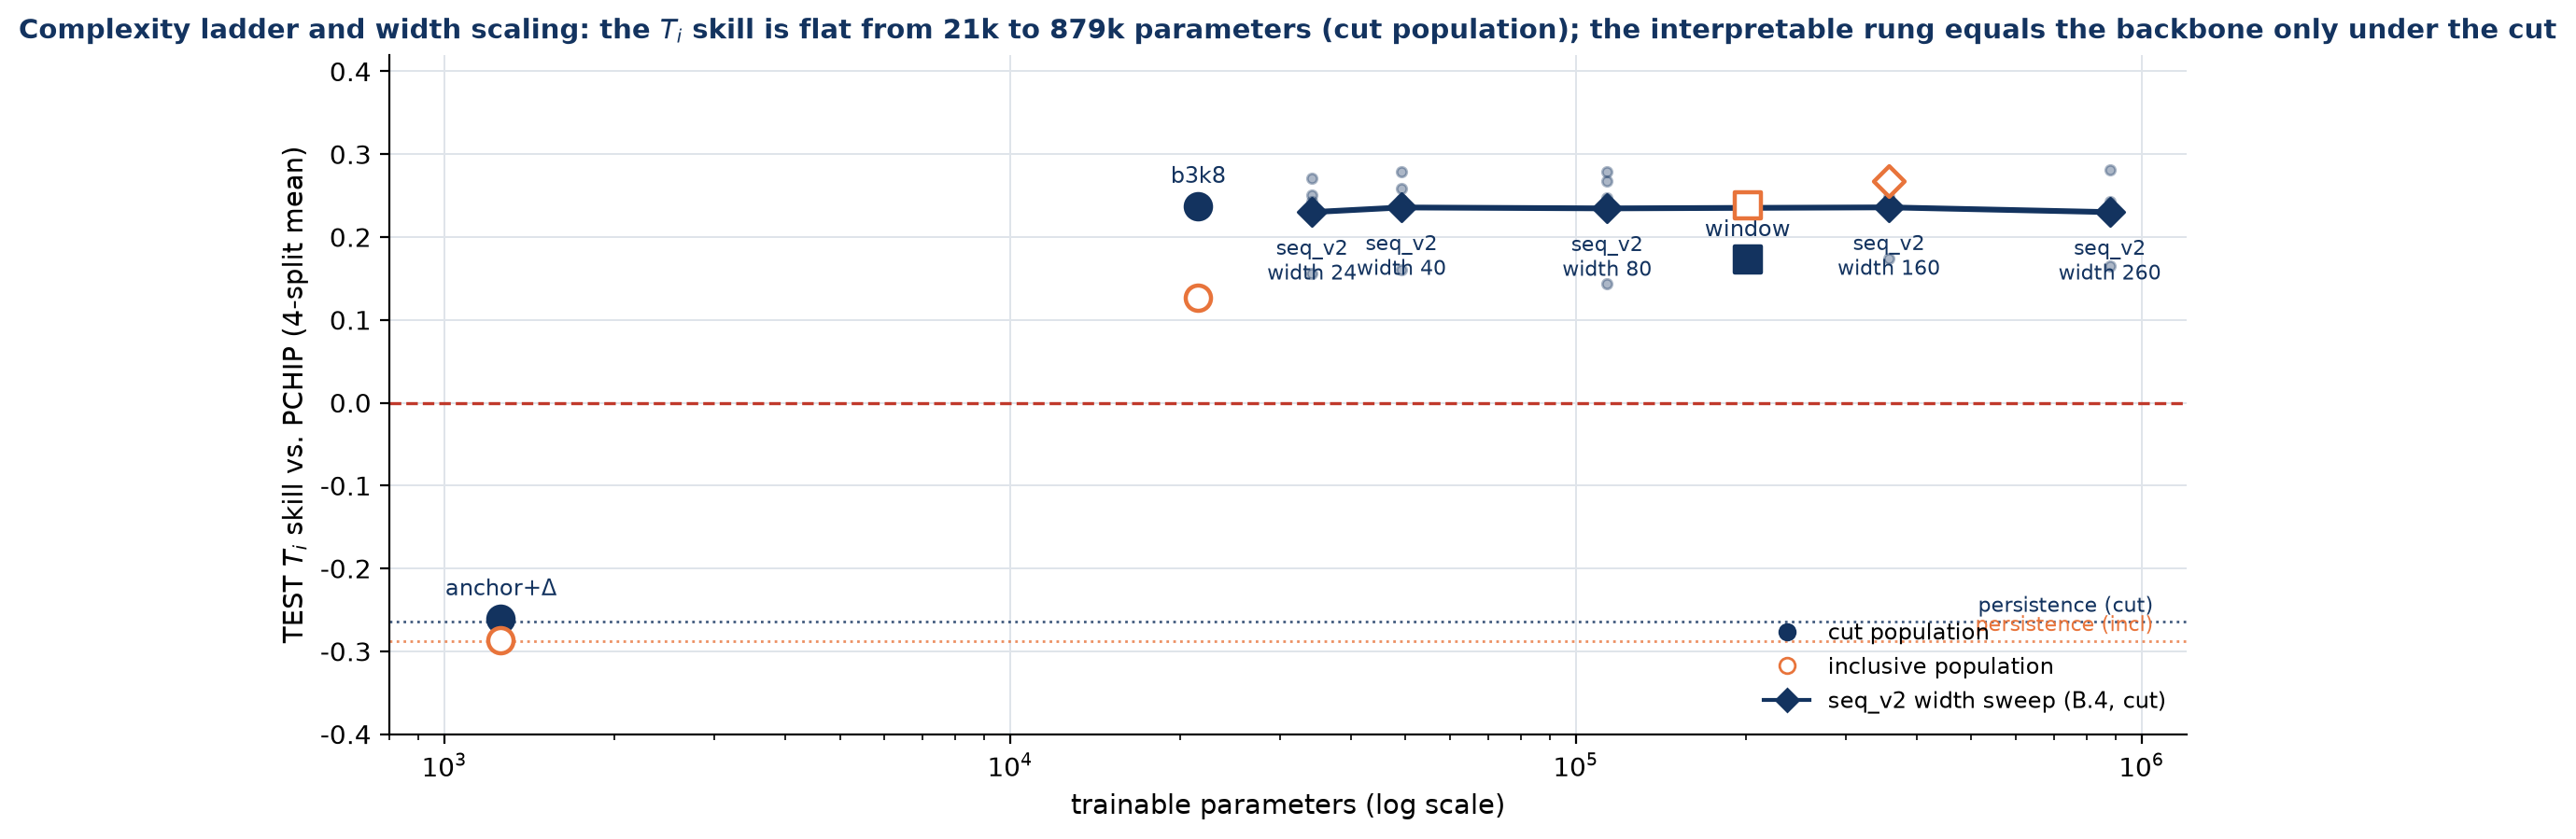
\includegraphics[width=0.95\linewidth]{fig_ladder_scaling}
  \caption{복잡도 사다리와 폭 스윕을 한 축에 놓은 그림(TEST \Ti{} skill 대 학습
  가능 파라미터 수, 4개 분할 평균). 컷에서는 21k 잠재 병목 모델이 백본의 곡선 위에
  놓이고 곡선은 34k에서 879k 파라미터까지 평평하다. 포함 모집단에서는 유계 보정
  사다리 칸이 $+0.126$으로 떨어진다.}
  \label{fig:ladder_scaling}
\end{figure}

\begin{itemize}
  \item \textbf{컷에서는 백본의 \Ti{} skill 전부가 유계 수 여덟 개와
        persistence로의 압축을 견딘다.} \bthree{}는 \Vrot{} 손실 없이 4/4
        분할에서 재학습된 앵커를 이기고, 백본에 대한 짝지은 \Ti{} skill은
        $-0.009$, $-0.005$, $+0.026$, $-0.004$이다(평균 $+0.002$, 모든 CI가 0을
        포함). PCHIP 대비 PR4를 4/4로 통과하고 인과 GP도 4/4로 이긴다. TEST
        입력에 대한 선형 probe(타겟은 건드리지 않음)는 \Ti{} 잠재가 마지막 관측
        \Ti{}($R^2$ 0.47--0.75)와 ECEI $T_e$ 대리 지표(0.31--0.48)를 여러 차원에
        분산해 부호화하며, 국소 BES 활동(0.09--0.13)이나 경과시간(0.01--0.07)은
        거의 부호화하지 않음을 보인다. 학습된 보정은 예측 분산의 25--39\%를
        설명한다. 이 과제에 필요한 것은 전체격자 인과 상태이며, 그 상태는 작다.
  \item \textbf{컷이 없으면 이 사다리 칸은 백본 대비 $-0.16\sim-0.21$을
        치르고(4/4 유의) 3/4 분할에서 윈도 대조군 아래에 놓인다} --- 잠재 여덟
        개가 너무 적어서가 아니라, 유계 보정으로는 스파이크가 낀 이월값을 복구할
        수 없기 때문이다: persistence 오차가 2\,keV를 넘는 행은 포함 모집단 test
        행의 0.6--1.3\%인데 \bthree{}의 \Ti{} 제곱오차의 73--83\%를 담는다(PCHIP을
        포함한 다른 모든 팔에서도 70--83\%다). 사다리 칸 조건은 거기서도
        성립하지만(앵커 대비 4/4) 백본 허용 조건은 컷 조건부이며, 우리는 그렇게
        진술한다.
  \item \textbf{용량을 더 사도 얻는 것이 없다.} \seqv{}의 \Ti{} 인코더를 24에서
        260 유닛으로 넓히면(34k / 49k / 114k / 358k / 879k 파라미터, 다른 설정은
        전부 고정, 지점마다 TEST 1회) \Ti{} skill 평균은 $+0.230$ / $+0.236$ /
        $+0.235$ / $+0.236$ / $+0.230$(컷)이고, 358k 백본에 대해 짝지은 평균은
        $\pm 0.008$ 이내이며, 가장 넓은 지점이 유의하게 나은 것은 1/4 분할,
        24 유닛까지 내려가도 $\geq$3/4에서 유의하게 나쁜 폭은 없다. \Vrot{}은
        (분기가 고정되어) 움직이지 않는다($+0.250\sim+0.254$). 사다리 칸과 함께
        이것은 모델 크기 축을 닫는다: \{100\,Hz BES/ECEI/MC + CES 이력 + 시간\}에
        든 \Ti{} 정보는 $\sim$50k 파라미터의 인과 순환 상태로 소진되며, 분할 간에
        남는 분산(시드 42의 $+0.14\sim+0.17$ 대 시드 123의 $+0.23\sim+0.28$)은
        용량이 아니라 분할 분산이다.
\end{itemize}

\subsection{우위는 고변동 국소 구간에 집중된다}
\label{sec:peak}
타겟과 무관한 입력 측 국소 활동 대리 지표(이웃 괄호 기울기가 크거나 국소 CES
이웃 분산이 높음, 타겟 행을 \emph{제외}하고 계산)를 사용해 각 TEST 분할을
``peak''(고활동; 분할당 \Ti{} 4.1--4.6k행, \Vrot{} 2.4--2.9k행)와 bulk 행으로
나누고, 각각에서 shot 군집 bootstrap으로 \seqv{}를 채점한다(그림~\ref{fig:peak}).

\begin{itemize}
  \item \Ti{}: peak 계층 $\skillp$는 컷에서 $+0.45\sim+0.61$, 포함에서
        $+0.62\sim+0.72$이며, 미래 이웃을 가진 보간기를 상대로 \textbf{8/8
        PASS}다. bulk는 컷에서 $+0.09\sim+0.20$(PASS 4/4), 포함에서
        $+0.06\sim+0.19$(PASS 2/4)를 담는다. 매끄러운 bulk에서는 보간이 거의
        최적이며, 모델의 가치는 활동 구간에 있다 --- 그리고 이 진술은 무조건적이다.
  \item \Vrot{}: peak 계층 skill은 $+0.54\sim+0.79$(8/8에서 점추정 양수, 각
        모집단에서 PASS 2/4, persistence 대비로는 $+0.75\sim+0.86$에 8/8 PASS)이고
        bulk에서는 $\approx 0$이다($-0.07\sim+0.15$, PASS 0/8). 따라서 비대칭은
        \emph{지역적}이다: 전역적으로 \Vrot{}은 보간과 동률이지만, 매끄러운
        과거+미래 보간이 가장 나쁜 고활동 국소 구간에서는 이력 기반 \Vrot{}
        예측기조차 가치를 더한다. 이를 전역 영가설의 뒤집힘이 아니라 유의성
        기반이 얇은 지역적 강점으로 보고한다.
\end{itemize}

\begin{figure}[t]
  \centering
  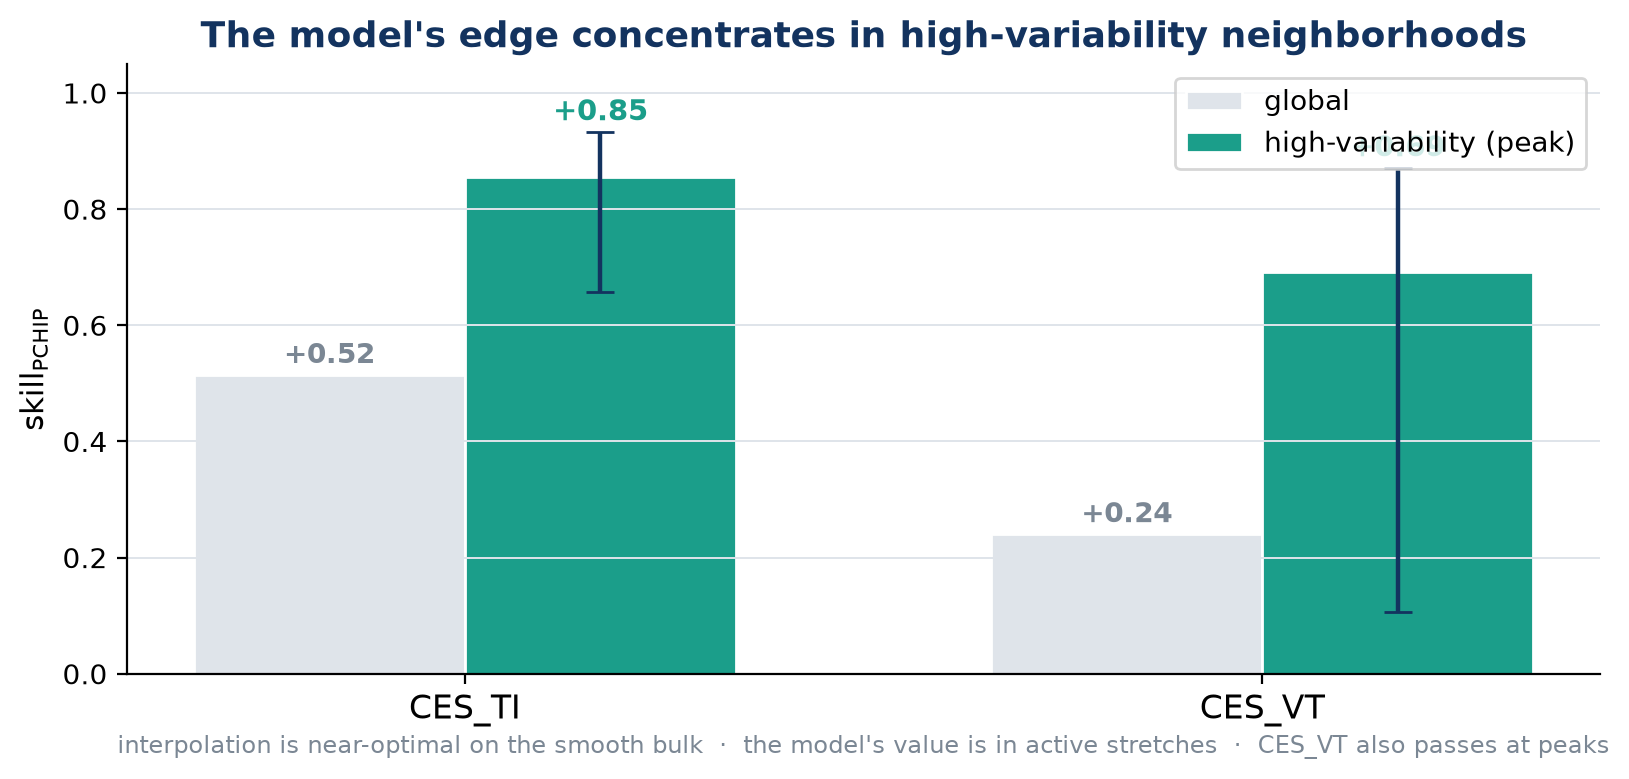
\includegraphics[width=0.9\linewidth]{fig_peak}
  \caption{\seqv{}의 peak 계층별 TEST skill, 두 모집단(4개 분할 평균, 분할별 점,
  PR4 카운트). 보간 대비 우위는 보간이 가장 약한 곳에 집중되며, \Vrot{} skill은
  전적으로 peak 계층에 산다.}
  \label{fig:peak}
\end{figure}

\subsection{컷 임계값 민감도}
\label{sec:cutsens}
스파이크 임계값을 2.5와 4\,keV로 두고 백본을 재학습하면(각각 4개 분할, 자기
모집단에서 채점) \Ti{} skill 평균이 $+0.230$과 $+0.232$로 3\,keV의 $+0.236$에
대응하고, 모든 임계값에서 PCHIP 대비 PR4 4/4, 인과 GP 대비 4/4이며, \Vrot{}은
$+0.252$ / $+0.253$ / $+0.257$이다. 물리학자가 방어할 만한 범위 안에서 임계값은
무의미하다. 중요한 것은 꼬리 안의 어디에서 자르느냐가 아니라 두 모집단이다.

\subsection{문맥·구조·비용: 무엇이 skill을 정하고 무엇이 값을 정하는가}
\label{sec:context}

앞의 결과들은 하나의 아키텍처를 하나의 문맥 길이 위에서 채점한다. 이 절은 그 둘을
따로 움직여 어느 쪽이 결과를 만드는지를 가른다. 두 축은 서로 크게 다른 답을 준다:
\emph{문맥}을 20\,ms에서 630\,ms로 늘리면 \Ti{} skill이 $+0.055$에서 $+0.138$로
오르지만, 같은 문맥에서 \emph{계열}을 순환에서 확장 합성곱이나 attention으로
바꾸면 어디에서도 0.023을 넘지 못한다. 그러므로 아키텍처는 skill이 아니라 비용으로
정해야 하며, 그 비용은 파라미터 수가 아니라 디스패치되는 연산자 수에서 나온다.

\paragraph{도달 범위는 절단이 아니라 학습으로 재야 한다.}
학습된 백본의 순환 상태를 사후에 $r$ 스텝으로 자르면 \Ti{}는 500\,ms까지 손해를
보는 것처럼 보이지만, 이는 정보 부족이 아니라 \emph{학습되지 않은 상태 재구축}을
정보로 잘못 읽은 것이다. 각 $r$에서 잘라 낸 비중첩 세그먼트로 \emph{다시 학습}하면
그 결손의 최소 84\%가 회복된다. 이하의 모든 도달 범위 수치는 절단이 아니라
각 문맥에서 학습된 모델의 것이다.

\paragraph{약 50\,ms에서 포화하며, 문맥이 사는 것은 평균이 아니라 전형성이다.}
사전등록된 규칙(전체 문맥 대비 결손이 0.02 미만이고 유의한 결손이 4개 분할 중
1개 이하인 가장 작은 $r$)을 한 스텝 간격으로 밀집시킨 사다리에 적용하면
\textbf{5스텝 = 50\,ms}가 반환된다. 그러나 이를 ``이겨야 할 문턱''으로 읽으면 안
된다. 4개 분할을 방전 단위로 통합해 301개 방전 위에서 재채점하면
표~\ref{tab:pooled}가 되고, \textbf{모델은 20\,ms에서도 인과 GP를 이긴다}
($+0.057$, 95\,\% CI $[+0.027, +0.085]$).

\begin{table}[t]
  \centering
  \caption{순환 계열, 301개 방전 통합 재채점. ``승률''은 인과 GP를 이긴 방전의
  비율, ``$-$상위10''은 기여가 큰 방전 10개를 지운 뒤의 통합 skill이다. 문맥 10배당
  추세는 $+0.0497$ $[+0.0363, +0.0638]$로 상승한다.}
  \label{tab:pooled}
  \small
  \begin{tabular}{rccc}
    \toprule
    문맥 & \Ti{} skill vs 인과 GP [95\,\% CI] & 승률 & $-$상위10 \\
    \midrule
    20\,ms  & $+0.057$ $[+0.027, +0.085]$ & \textbf{0.52} & $+0.028$ \\
    30\,ms  & $+0.087$ $[+0.061, +0.111]$ & 0.60 & $+0.060$ \\
    50\,ms  & $+0.104$ $[+0.079, +0.128]$ & 0.64 & $+0.077$ \\
    70\,ms  & $+0.119$ $[+0.095, +0.142]$ & 0.66 & $+0.092$ \\
    150\,ms & $+0.123$ $[+0.096, +0.148]$ & 0.66 & $+0.096$ \\
    630\,ms & $+0.143$ $[+0.118, +0.168]$ & 0.67 & $+0.116$ \\
    \bottomrule
  \end{tabular}
\end{table}

승률 열이 이 절의 결론이다: $0.52 \rightarrow 0.60 \rightarrow 0.64 \rightarrow
0.66$으로 오른 뒤 약 70\,ms부터 평평하다. 20\,ms에서 모델은 평균으로는 이기지만
방전의 절반에서만 이기고, 70\,ms에서는 3분의 2에서 이긴다. \textbf{문맥은 평균을
올린다기보다 승리를 전형적인 것으로 만든다.} 이것이 배치를 판단하는 쪽이 필요로
하는 진술이며, 문턱을 ``유용해지기 위해 필요한 문맥''으로 기술해서는 안 된다:
20\,ms에서도 모델은 배치된 시스템이 실제로 대체하는 persistence를 $+0.356$으로
앞선다.

한 가지 방법론적 주의를 이 사다리가 강제한다. 분할별 4/4 계수는 한 스텝 간격에서
도달 범위의 단조 함수가 아니다(20--630\,ms에서 $2/4 \rightarrow 3/4 \rightarrow
4/4 \rightarrow 3/4 \rightarrow 4/4 \rightarrow 4/4 \rightarrow 3/4 \rightarrow
4/4 \rightarrow 4/4 \rightarrow 4/4$). 그 아래의 점추정은 매끄럽게 오르므로,
이는 4개 표본에 대한 5단계 투표의 성질이지 실행의 문제가 아니다. 계수는 보고하되
판정은 결손으로 한다.

\paragraph{같은 문맥에서 계열은 skill을 정하지 않는다.}
도달 범위를 맞춘 채 순환 LSTM(357{,}570 파라미터), 확장 인과 합성곱(3{,}238),
띠 attention(295{,}746)을 비교하면 셋 다 인과 GP를 4/4로 이기고 그 값은
$+0.113$ / $+0.119$ / $+0.119$이다. 110배의 파라미터 범위와 서로 가장 다른 세
시퀀스 연산자가 구별되지 않는 결과를 낸다. 사다리로 보면 표~\ref{tab:family}이며,
같은 도달 범위에서 짝지어 비교하면 차이는 더 조용하다: \texttt{tcn3/5/7}은
같은 도달 범위의 LSTM과 동률이고($-0.004$, $+0.005$, $-0.004$; 어느 쪽으로도
유의한 분할 없음), attention만 70\,ms 칸에서 $-0.023$(3/4 유의)으로 사전등록 규칙이
``차이''를 반환한다. 어디에서든 계열이 \Ti{}를 움직이는 폭은 최대 0.023이고,
도달 범위를 20에서 70\,ms로 옮기는 효과는 $+0.060$이다.

\begin{table}[t]
  \centering
  \caption{계열별 도달 범위 사다리(\Ti{} skill vs 인과 GP, 4개 분할 평균 · CI가 0을
  제외한 분할 수). 본 연구의 승격 기준 $\ge 3/4$ 위에서 세 계열 모두 단조이다.
  합성곱 팔의 30\,ms는 구조적 최소(1층, 수용영역 3)이므로 그 교차점은 상한이다.}
  \label{tab:family}
  \small
  \begin{tabular}{rlll}
    \toprule
    문맥 & 순환(LSTM) & 확장 합성곱(TCN) & 띠 attention \\
    \midrule
    20\,ms  & $+0.055$ · 2/4 & --- & --- \\
    30\,ms  & $+0.083$ · 3/4 & $+0.079$ · 3/4 & --- \\
    50\,ms  & $+0.098$ · 3/4 & $+0.103$ · 3/4 & $+0.090$ · 2/4 \\
    70\,ms  & $+0.115$ · 4/4 & $+0.111$ · 4/4 & $+0.094$ · 3/4 \\
    150\,ms & $+0.117$ · 4/4 & $+0.130$ · 4/4 & $+0.119$ · 4/4 \\
    630\,ms & $+0.138$ · 4/4 & $+0.124$ · 4/4 & $+0.122$ · 4/4 \\
    \bottomrule
  \end{tabular}
\end{table}

네 번째 계열인 대각 상태공간 모형(SSM)은 같은 사다리 위에서 다르게 행동한다.
문맥을 skill로 바꾸기는 하지만($+0.0235$ / 문맥 10배 $[+0.0102, +0.0372]$) 약
70\,ms에서 멈추고 더 낮은 천장에 머문다: 630\,ms에서 $+0.105$로 순환의 $+0.143$에
못 미치고 승률도 0.58--0.60에서 0.66에 이르지 못한다. 다만 20\,ms 통합 점수에서는
어느 계열보다 좋다($+0.065$ 대 순환 $+0.057$) --- 같은 칸의 통합 비교이지 짝지은
검정이 아니므로 보고만 하고 승격하지 않는다. \Vrot{}은 \textbf{네 계열 모두에서}
문맥이 길어질수록 나빠진다.

\paragraph{그러므로 아키텍처는 비용으로 정하며, 비용은 연산자 수이다.}
온라인 1스텝의 지연은 파라미터 수나 부동소수점 연산량이 아니라 디스패치되는
연산자 개수를 따라간다(약 2--3\,$\mu$s/연산자). 그 개수는 기계와 무관하게 정확하며,
이 기계의 절댓값은 5개 세션 사이에서 21.84배로 흔들렸으므로 인용하지 않는다.

\begin{table}[t]
  \centering
  \caption{계열별 온라인 1스텝 비용. $R$은 도달 범위, ``ops''는 스텝당 디스패치되는
  \texttt{aten::} 연산자 수이다. attention도 KV 캐시 덕분에 $R$에 대해 $O(1)$이지만
  상수가 3.5--4.3배 나쁘다.}
  \label{tab:cost}
  \small
  \begin{tabular}{llrr}
    \toprule
    계열 & $R$에 대한 비용 & $R=15$ & $R=63$ \\
    \midrule
    순환(LSTM) & $O(1)$ --- 상태가 나른다 & 111 & 111 \\
    확장 인과 합성곱 & $O(\log R)$, 층당 $+48$ & 209 & 305 \\
    띠 attention & $O(1)$, 상수 4.3배 & 473 & 473 \\
    \bottomrule
  \end{tabular}
\end{table}

이 문제에서 attention은 \emph{엄밀히 지배당한다}: \texttt{tcn3k}(3{,}238 파라미터)가
같은 skill($+0.119$, 4/4)을 91배 적은 파라미터와 2.3--2.7배 적은 연산자로 낸다.
이름 붙일 만한 운용점은 셋이다 --- \texttt{tcn3k}는 357{,}570 파라미터 백본과
\Ti{}에서 동급이고 인과 GP를 4/4로 이기며, \texttt{v2m4k}(3{,}898)는 4/4를 유지하는
가장 싼 순환 팔, \texttt{tcn2k}(1{,}808)는 계열을 통틀어 가장 싼 팔이다. 이들은
``모델의 축소판''이 아니라 이 문제가 실제로 요구하는 것의 답이다. 10\,ms 예산은
어느 팔에도 구속 조건이 아니며, 1\,ms 판정은 위의 세션 간 산포 때문에
사전등록 규칙에 따라 \textbf{보류}되었다.

\paragraph{윈도 계열이 이 축에 닿을 수 없었던 이유.}
\S\ref{sec:window}는 과거 \emph{관측} 하나면 충분하다고 보고했고 이 절은 약 50\,ms의
\emph{연속 문맥}이 필요하다고 보고한다. 둘은 다른 자원을 세므로 충돌하지 않는다.
윈도 계열은 첫 번째를 만족했지만 두 번째에는 어떤 $W$에서도 도달할 수 없었다:
윈도를 평균 풀링하면 순서가 버려지고, 시간적 부분집합 증강은 각 윈도를 과거 행의
임의의 비연속 부분집합으로 만들며, 타겟이 관측되지 않은 행은 모델이 보기 전에
버려진다. 수치가 정확히 그 설명이 예측하는 자리에 놓인다: $W{=}2$의 윈도 모델은
인과 GP 대비 $+0.041$(1/4)이고, 같은 2스텝으로 자른 \seqv{}는 $+0.055$(2/4)이다.
서로 다른 아키텍처, 같은 결핍, 같은 결과다. 전체격자 재프레이밍은 모델링 취향이
아니라 문제가 요구하는 자원에 도달하는 유일한 방법이었다.

\paragraph{모델은 타겟이 움직이는 방전에서 이긴다.}
통합 재채점은 \Vrot{}에 대해 홀로 읽으면 오독될 결과를 낸다: 모든 칸의 통합 CI가
0을 제외한다(예: 70\,ms에서 $+0.123$ $[+0.036, +0.248]$). 그러나 방전 단위 승률은
0.48이고 중앙 방전의 skill은 약 0이며, 약 62개 방전 중 상위 5개를 제거하면 네 분할
모두에서 통합 우위가 0 이하로 내려간다. \textbf{좁은 구간은 일반적 효과와 같지
않다.} \Ti{}는 반대다: 방전의 70\%에서 이기고 상위 1개 방전의 기여 비중이 9--16\%에
그친다.

승패를 예측하는 공변량을 11개 검사한 결과 살아남은 것은 하나뿐이며, 그것은
\emph{방전 안에서 타겟이 얼마나 움직이는가}이다. 그 산포의 3분위로 나누면 \Ti{}의
승률은 42\,\% / 83\,\% / 85\,\%, \Vrot{}은 34\,\% / 48\,\% / 55\,\%이다. 메커니즘은
통계적이 아니라 물리적이다: 방전이 평평한 곳에서는 인과 GP가 이미 최적에 가깝고
직선을 보간하는 일에 모델이 더할 것이 없다. 그리고 \Vrot{}이 가장 변동이 큰
3분위에서조차 55\,\%에 그친다는 사실은 \S\ref{sec:model:physics}의 항별 감사를
반대편에서 다시 말한 것이다 --- 회전의 구동 변수가 관측되지 않으므로, 모델은
입력이 없는 운동을 따라갈 수 없다. 계열의 선호도 같은 방향을 가리킨다: \Vrot{}에
가장 좋은 팔은 작은 \emph{순환} 팔이고 \Ti{}에 가장 좋은 팔은 작은 \emph{합성곱}
팔인데, 이는 \Vrot{}이 강하게 자기상관된 이월값을 타므로 순환이면 족하고 \Ti{}는
고속 진단 이력을 적분하므로 시간에 걸친 가중치 공유가 값을 한다는 라우팅의 예측
그대로다.

% =========================================================================
\section{모델 선택 프로토콜}
\label{sec:selection}

본 논문의 모든 모델 결정은 검증 데이터 위에서, 또는 해당 TEST 채점 이전에 문서로
확정된 결정 규칙 아래에서 이루어졌고, TEST는 결정마다 한 번만 채점되었다.

\paragraph{윈도 계열.} 그 아키텍처는 통제된 실험의 연속으로 도달했다. 각 실험은
데이터 계약을 보존해야 하는 \emph{하나의} 변경이었고, \emph{깨끗한 비증강} 검증
$\skillp$로 채점되었으며---증강된 검증 손실은 보간이 이미 강한 바로 그곳에서
평활화를 보상하므로 결코 쓰지 않았다---지금까지의 최고 점수를 개선할 때만
유지되었다. 이후 이력 길이는 \S\ref{sec:window}의 스윕으로 정해졌고, 유지값은
\S\ref{sec:stuck}의 감사에 따라 학습에서 제거되었다.

\paragraph{백본 관문.} 시퀀스 프레이밍은 \S\ref{sec:gate}의 네 조건 관문(4/4
분할에서 부호 유지, 통합 실행 군집 CI가 0을 제외, 예산 균등화에서도 부호 유지,
\Vrot{} 손실 없음)이 먼저 고정되고 그 다음 충족된 뒤에야 채택되었다. 같은 규칙
아래에서 이후 탐색된 단 하나의 아키텍처 후보---각 타겟 자신의 과거 관측 스텝에
대한 관측 마스킹 인과 어텐션을 0으로 초기화된 사영과 함께 \seqv{}에 추가한
것---는 4/4 분할에서 양수였으나(백본 대비 $+0.009$, $+0.013$, $+0.033$,
$+0.020$) $\geq 3/4$라는 사전 확정 기준에 대해 1/4에서만 유의했으므로
\emph{승격되지 않았고}, 백본은 \seqv{}로 남았다. 이 후보의 검증 이득은 탐색
분할에서 2/2 유의했는데, 이는 선택 분할 결과의 통상적 낙관이며 승격 기준을
TEST에 두는 이유다.

\paragraph{사다리 칸과 폭 스윕}(\S\ref{sec:ladder})은 두 갈래 판정과 서술적
독법(천장 / 무릎)을 어떤 TEST 채점 이전에 적어 두었고, 구성상 이 스윕 위에서
백본을 재선택하는 것은 허용되지 않았다. 전체 사전등록 문서와 배치별 실행 기록,
러너 스크립트는 공개 저장소에 있다.

% =========================================================================
\section{배치 가능한가?}
\label{sec:deploy}

skill 점수와 쓸 만한 계측기 사이에는 두 가지가 놓여 있다. 측정 주기 안에서
돌아야 하고, 얼마나 믿어도 되는지를 말할 수 있어야 한다.

\paragraph{지연시간: 상태 유지형 1-스텝 추론은 여유를 두고 CPU에 들어간다.}
CES는 10\,ms 격자 위에 있으므로 온라인 결측 채움기는 한 스텝당 10\,ms에서 획득과
제어가 이미 쓰는 몫을 뺀 시간을 갖는다. 순환 나우캐스터는 온라인에서 \emph{상태를
유지한 채} 실행된다: 은닉 상태가 격자를 따라 이월되고 새 행마다 배치 1의 순환
스텝 하나가 드는데, 이것이 실제로 중요한 수치다. 유휴 상태의 노트북급 머신에서
워밍업 후 1{,}000회 호출을 계측해 네트워크 순전파만(특징 조립은 모델 밖이다) 잰
값으로, \seqv{} 스텝은 \textbf{CPU에서 중앙값 1.05\,ms, p99 1.61\,ms}(격자 주기의
16\%; p95 1.35\,ms), GPU에서 1.21 / 2.31\,ms이다---이 크기에서 GPU는 배치 1에서
아무것도 사주지 않는다. 오프라인 채점이 쓰는 세그먼트 전체 재실행은 CPU에서
100행(1\,s) 블록당 중앙값 2.9\,ms / p99 5.6\,ms, 300행당 6.4 / 8.9\,ms, 즉 대량
재처리 기준 35--47k 행/s(GPU 47--63k 행/s)이다. 배치 1의 윈도 대조군은 더 느리고
이 머신에서는 꼬리가 무겁다: $W{=}2$는 CPU 중앙값 3.8\,ms이지만 p99 18.9\,ms(GPU
7.2 / 11.6\,ms), $W{=}4$는 4.0 / 8.1\,ms. 같은 벤치마크를 유휴 상태에서 두 번
돌린 결과는 절대값에서 최대 2$\times$ 차이가 났고(다른 실행에서 \seqv{} 스텝은
중앙값 / p99 0.51 / 0.99\,ms), 노트북의 전원 상태가 이 수치를 움직이기 때문이지만
순서---시퀀스 스텝 $\ll$ 윈도 순전파, CPU로 충분---는 바뀌지 않았다. 따라서 실무
지침은 \emph{상태 유지형 나우캐스터를 제어 계산기의 CPU에서 돌리라}는 것이며,
10\,ms 예산의 80\% 이상이 획득과 제어에 남는다.

\paragraph{불확실성: 모델을 건드리지 않는 분포 무가정 구간.}
핵융합 프로파일 데이터의 커뮤니티 표준은 사후분포를 돌려주는 가우시안 과정
회귀이고, 우리 모델은 점추정을 돌려준다. 분산 헤드나 분위 헤드를 붙이면 재학습이
필요하고 위의 모든 수치가 움직이므로, 대신 \emph{split conformal prediction}을
쓴다: 해당 실행 자신의 검증 분할에서 보정하고, 예측기는 아무것도 바꾸지 않으며,
분포 무가정 유한표본 주변 커버리지를 얻는다. 변형은 둘이다: 단일
분위(\emph{global})와 $\Delta t$ 구간별 분위(\emph{Mondrian}). 동일한 절차를
PCHIP과 persistence에도 적용하므로 비교되는 것은 보정 기법이 아니라 구간의
품질이다. $\alpha = 0.10$, TEST, 두 모집단에서:

\begin{itemize}
  \item \textbf{모델의 구간이 모든 셀에서 두 기준선의 구간을 이긴다}(32/32
        모집단 $\times$ 타겟 $\times$ 변형 $\times$ 분할). 폭과 빗나감을 함께
        벌하는 Winkler 구간 점수 기준으로 컷 모집단의 \Ti{}는 1{,}272 대
        1{,}554(PCHIP) 대 1{,}727(persistence), 포함 모집단은 2{,}290 대
        2{,}851 대 3{,}120이며, \Vrot{}은 150 대 164 대 179이다(global 변형,
        4개 분할 평균). 이는 더 나은 점추정에서 따라 나오는 것이 아니라 별개의
        성질이다.
  \item \textbf{포함 모집단에서 모델의 \Ti{} 구간은 실제로 PCHIP의 것보다
        \emph{넓은데}}(반폭 224--255 대 211--241\,eV) 그럼에도 점수는 더 좋다:
        스파이크가 빗나감 벌점을 부풀리는데 모델이 덜 빗나가기 때문이다. Mondrian
        보정은 모든 \Ti{} 팔을 $\approx$4--5\% 좁히고 \Vrot{}은 그대로 두며 어떤
        판정도 바꾸지 않는다.
  \item \textbf{정직한 실패: 커버리지는 주변적이지 조건부가 아니다.} \Ti{}
        커버리지는 목표 $0.90$에 대해 $0.87$--$0.92$이고(모든 팔에서 한 분할이
        미달) \Vrot{}은 $0.91$--$0.94$이며, shot별 커버리지는 여전히 넓게
        흩어진다. Conformal은 교환가능성 아래에서 커버리지를 보장하는데, 보정과
        test는 서로소인 \emph{방전}이다. shot 수준의 이동이 그 가정을 깬다. 배치된
        계측기에는 통합 수치보다 이것이 더 중요하며, 이를 고치려면 현재 shot 수로는
        지탱할 수 없는 shot 조건부 보정이 필요하다.
\end{itemize}

% =========================================================================
\section{남은 개선 여지는 어디인가}
\label{sec:headroom}

본 논문의 부정 결과들은 이례적으로 구체적이며, 그 구체성이 그것들을 쓸모 있게
만든다: ``이 문제는 어렵다''가 아니라 \emph{어떤 변경이 이를 움직일지}를 말한다.
용량은 배제되었고(\S\ref{sec:ladder}), 더 긴 윈도도 배제되었으며
(\S\ref{sec:window}), 도달 범위를 사는 프레이밍은 채택되었다(\S\ref{sec:gate}).
남은 것은 데이터이고, 각 레버는 이미 이 데이터셋 안에 있는 증거로 지목된다.

\paragraph{1. CES 피팅 품질 메타데이터는 대리 지표를 측정으로 대체할 것이다.}
두 모집단 보고가 존재하는 이유는 값 기준 컷이 ``피팅이 실패했다''의 대리 지표이기
때문이다: 어떤 방법도 예측할 수 없는 단일 표본 상향 사건을 제거하지만 한쪽
방향뿐이고(하향 급락은 손대지 않는다) $\geq 2\times$ 상향 이상치의 19\%만
잡는다(\S\ref{sec:spikes}). 표본별 피팅 $\chi^2$이나 신호 수준이 있다면 품질 컷이
모든 팔에서 한꺼번에 값 컷을 대체하거나 동반할 수 있고, 두 모집단은 하나로 합쳐질
것이다. \Vrot{} 자신의 스파이크(1{,}000\,km/s를 넘는 119행)도 같은 규칙으로
처리될 것이다. 그때까지 persistence 기반 \Vrot{} 비교는 \S\ref{sec:ladder}처럼 그
행들이 담는 제곱오차 비중을 보고한다.

\paragraph{2. Mirnov 정보는 플라즈마에 없었던 것이 아니라 전처리에서 파괴되었다.}
\S\ref{sec:asym}에서 자기 진단이 회전 정보를 운반하지 않는다고 결론짓는 것은
틀렸다. 동일한 10\,ms 격자에서 연속 블록 내 lag-1 자기상관은 BES가 $+0.568$,
ECEI가 $+0.572$인 반면 Mirnov 코일은 $-0.009$이고 블록의 82\%가
$|r| = 0.1$ 아래다: 이 격자 \emph{위에서} 자기 채널은 백색잡음이다. 이는
$\mathrm{d}B/\mathrm{d}t$가 kHz 모드 주파수로 진동하는 것을 앤티앨리어싱 필터
없이 100\,Hz로 데시메이션한 결과의 특징으로, 연속한 표본들의 상대 위상이
무작위가 된다. 우리 진단 집합에서 토로이달 회전의 대리가 될 수 있었던 유일한
물리량인 모드 회전 주파수가 모델보다 상류에서 버려진 것이며, 우리가 시도한 모든
파생 MC 특징(적분, PCHIP 적분, $|MC|$, 이동 RMS)이 실패한 이유이기도 하다: 이미
잃은 정보는 하류에서 복구할 수 없다. 해결책은 모델 변경이 아니라 전처리 변경이다:
\emph{원시} kHz Mirnov 시계열에서 계산한 윈도별 RMS, 대역 파워, 모드 수, 모드 회전
주파수를 사전등록된 pilot-then-expand 규칙 아래 \Vrot{} 분기로 라우팅하는 것.
이것이 \Vrot{}에 대해 우리가 지목할 수 있는 가장 가치 높은 실험이며, 아카이브된
데이터로 검정 가능하다.

\paragraph{3. 액추에이터 채널이 아예 없다.}
토로이달 회전은 주입된 토크로 결정되는데, 이 데이터셋에는 토크 신호가 존재하지
않는다. 데이터가 그 단절을 정확히 보여준다: shot 사이에서 ECE 유래 $T_e$ 대리
지표는 \Ti{}와 $r = +0.353$($p = 3\times10^{-17}$)으로 상관되지만 \Vrot{}과는
$r = +0.024$($p = 0.58$)이고, shot 내부에서 \Ti{} 상관은 일관된 부호를 유지하는
반면 \Vrot{} 상관은 부호가 무작위다. 즉 $T_e$는 가열 수준을 추적하지만 가열
수준은 회전에 닿지 않는다---파워는 토크가 아니며, 토크는 빔 에너지, 접선 반경,
주입 기하에 의존한다. NBI 토크(또는 그것을 계산하는 빔별 파워와 기하)를 더하는
일은 모델링 과제가 아니라 데이터 획득 과제이고, 회전의 자기상관이 아니라
\emph{원인}을 다루는, 우리가 지목할 수 있는 유일한 레버다. 문헌에 이미 양성
대조가 있다: 빔 액추에이터를 입력으로 받는 DIII-D의 순환 전방전
시뮬레이터는 회전의 시간 변화를 예측한다~\citep{Char2024FullShot}. 따라서 없는
채널은 측정되기만 하면 학습 가능하다.

이들 중 어느 것도 현재 결과가 천장에 있다는 진술이 아니다. 이들은 다음의 측정
가능한 이득이 있는 자리를 값싸게 시도할 수 있는 순서로 늘어놓은 것이며, 셋 모두
아카이브된 KSTAR 데이터에서 실행 가능하다.

% =========================================================================
\section{한계}
\label{sec:limits}

\textbf{통계적 검정력.} 재현의 단위는 shot이며, 분할당 test shot이 96개(\Ti)
/ 60--66개(\Vrot)이므로 검정력이 모든 유의성 판정을 제약하고, shot별 제곱오차
차이는 두꺼운 꼬리를 갖는다(소수의 방전이 bootstrap 산포를 지배한다. 포함
모집단에서는 행의 $\approx$1\%가 모든 팔의 \Ti{} 제곱오차의 70--83\%를 담는다).
\textbf{MNAR 낙관.} skill은 관측 지점에서만 측정된다. \S\ref{sec:mnar}의 재가중은
두 모집단 모두에서 인과 비교에 대한 낙관의 상한을, 오프라인 비교에 대해서는
모집단 조건부 유의성으로 그 상한을 정하며, 결측 \Ti{} 행의 54--68\%와 결측
\Vrot{} 행의 4--6\%를 포괄한다.
\textbf{오프라인 주장의 상한은 GP 동률이다.} 오프라인 GP는 PCHIP을 이기고 모델은
그것과 동률일 뿐이므로(8개 셀 중 1개 유의), ``미래를 쓰는 보간을 이긴다''는
``사전등록된 보간들을 이긴다''를 뜻하며 모든 오프라인 방법으로 확장되지 않는다.
다만 배치 가능한 가장 강한 방법인 인과 GP로는 확장된다.
\textbf{값 기준 컷은 대리 지표다.} 두 모집단이 피팅 실패 문제를 괄호로 묶지만,
이를 결말짓는 것은 피팅 품질 컷이며(\S\ref{sec:headroom}), \Vrot{}의 스파이크는
컷되지 않은 채로 남는다.
\textbf{캠페인 전이는 하나의 시간 블록에 기댄다}(\S\ref{sec:campaign}): 4개
분할이 아니라 4개 초기화이며, 컷 모집단 실행 4개 중 2개는 epoch 상한에서 멈췄다.
윈도 대조군을 전이시키는 수리인 shot별 표준화는 오프라인 형태이고, 실제로 출하될
버전인 인과적 러닝(확장 윈도/EWMA) 추정기는 여기서 측정되지 않았다.
\textbf{지표의 비대칭.} 보간은 shot 전체의 이웃을 쓰는 반면 윈도 대조군은 두 행을,
백본은 세그먼트의 과거를 본다. 이는 인과 모델에 의도적으로 불리하지만 직접적인
해석은 어렵게 만든다.
\textbf{단일 장치, 단일 모델 계열.} 모든 것이 하나의 장치, 하나의 진단 집합,
그리고 밀접하게 관련된 두 순환 계열에서 나왔다. 다른 토카막으로의 전이는 여기서
아무것도 확립되지 않았다.
\textbf{불확실성은 조건부가 아니라 주변적으로 보정된다}(\S\ref{sec:deploy}).
\textbf{지연시간}은 노트북급 머신 한 대에서 네트워크만 잰 값이며 전원 상태에 따라
실행 간 최대 2$\times$ 변동한다(\S\ref{sec:deploy}); 특징 조립과 획득 오버헤드는
포함되지 않는다.
\textbf{범위.} 페데스탈 상단 프레이밍은 데이터 선정(페데스탈 상단 CES 채널)에서
물려받은 것이며, 반경 의존성 실험은 수행하지 않았고 사건 위상 분석(ELM 주기,
L--H 천이)은 향후 과제다---\S\ref{sec:peak}의 고변동 분석은 사건에 무관한 대리
지표다.

% =========================================================================
\section{결론}
\label{sec:conclusion}

우리는 희소한 KSTAR CES 타겟을 위한 인과적·누수 방지 멀티모달 나우캐스터---
\Vrot{} 분기가 고속 진단을 결코 보지 않는 전체격자 2분기 순환 모델---를 만들고,
사전등록된 shot 군집 두-모집단 프로토콜 아래에서 의도적으로 불리한 기준
--- 미래를 보는 보간, 그리고 미래를 보지 않는 방법 중 가장 강한 인과 GP ---
에 대해 평가했다. 관측 모집단에서 모델은 이온온도에 대해 미래를 쓰는 PCHIP을
유의하고 재현 가능한 skill로 이기고(4개 독립 분할과 두 모집단에 걸쳐
$+0.17\sim+0.32$), 가장 강한 오프라인 평활기와 동률이며, 두 타겟 모두에서 모든
인과 기준선을 --- 8개 셀 전부의 인과 GP와 비인접 영역($\Delta t > 15$\,ms)을
포함해 --- 이긴다.

배치에 대한 우리의 주장은 이제 두 스트레스 테스트 모두의 지지를 받는다. 진짜
결측이면서 도메인 안인 시점에서 모든 인과 방법 대비 우위는 8/8 모집단--분할
셀에서 재가중을 견딘다. 캠페인 경계를 가로질러서는 시퀀스 나우캐스터가 두 모집단
모두에서 4/4 초기화에 대해 PCHIP과 인과 GP를 앞서는데, 그것이 대체한 윈도
대조군은 오프라인 우위를 완전히 잃었던 자리다. 그리고 그 차이는 단언이 아니라
측정이다: 고속 진단은 캠페인 사이에 타겟보다 5--11$\times$ 더 이동하고, shot별
표준화가 대조군을 수리하며, 시퀀스 프레이밍은 구성상 shot별로 표준화하고 과거
전체에 닿는다. 온라인 가상 센서는 미래를 읽는 보간이 아니라 persistence와 인과
평활기와 경쟁하며, 그 비교로 보면 나우캐스터는 중요한 지점에서 작동한다. 또한
모든 셀에서 적합한 채점 규칙으로 두 기준선의 구간을 이기는 보정된 구간을
내놓는다.

작동하지 않는 곳과 그 이유도 함께 보고한다. 회전은 전역적으로 보간과 동률이고 그
skill은 과도 구간에 산다. 두 모집단 중 하나를 정의하는 값 기준 컷은 피팅 품질에
대한 한쪽 방향 대리 지표다. 재가중은 결측 \Ti{} 행의 54--68\%와 결측 \Vrot{}
행의 20분의 1에 닿는다. 예측 구간은 방전별이 아니라 주변적으로 보정된다. 그리고
45\,ms를 넘어서면 포함 모집단은 동률이다. 이 중 어느 것도 천장 논변이 아니며,
어느 것도 어깨를 으쓱하는 것으로 남겨두지 않았다. 각각은 구체적이고 검정 가능한
변경을 가리킨다---CES 피팅 품질 메타데이터, 100\,Hz 데시메이션이 모델이 보기도
전에 파괴한 정보를 담고 있는 원시 kHz Mirnov 스트림에서 다시 계산한 윈도별 특징,
그리고 데이터셋에 없지만 회전의 물리적 원인인 NBI 토크 채널. 그리고 모델 크기 축은
닫혔다: 21k 파라미터의 persistence+유계 보정 모델이 컷에서 백본과 대등하고, 26$\times$
폭 스윕은 평평하다. 이와 함께 본 연구는 교정된 \Vrot{} 평가(54\%의 계측기 유지값,
전 구간 제거), 어느 한 모집단만으로는 왜 충분하지 않은지를 보이는 측정을 동반한
스펙트럼 피팅 실패의 두-모집단 처리, 배치 가능한 가장 강한 기준선을 넘어서게 하는
도달 범위를 지닌 전체격자 인과 프레이밍, 그리고 모든 결정 규칙이 그것이 결정할
수치보다 먼저 적힌 test 동결 선택 프로토콜을 기여한다.

% =========================================================================
\subsubsection*{재현성}
분할은 디스크에 고정되고 재적재 시 검증된다. 정규화 통계는 학습 파일
전용이다(시퀀스 계열은 여기에 shot별 입력 표준화가 더해진다). 모델 선택은 test
데이터를 결코 읽지 않는다. bootstrap은 고정 시드와 10{,}000회 재표본을 쓴다.
인용된 모든 수치는 단일 수집 스크립트가 동결된 평가 산출물에서 읽어온다.

\subsubsection*{코드 가용성}
전체 파이프라인, 배치별 실행 기록을 담은 사전등록 문서, 여기 보고된 모든 결과
뒤의 통제 실험 러너, 고정된 train/validation/test 분할, 그리고 동결된 평가
산출물에서 인용된 모든 수치를 재생성하는 수집기는
\url{https://github.com/iseungsang01/ml-intern-revision}에서 공개되어 있다.
백본은 \texttt{ces\_prediction/experiments/seq/model\_seq\_v2.py}, 해석 가능한
사다리 칸은 \texttt{model\_seq\_b3.py}, 윈도 대조군은
\texttt{ces\_prediction/model\_iter009.py}(테스트 스위트에서 내용 해시로 보호)이므로,
이 수치를 만든 코드가 공개된 코드와 어긋날 수 없다.
% TODO(user): mint an archival DOI (e.g. Zenodo) for the submitted revision and cite it here.

\subsubsection*{데이터 가용성}
본 연구의 바탕이 되는 KSTAR 진단 데이터---641개 방전, shot 30801--32751---는
코드와 함께 재배포되지 않는다. 이는 KSTAR 장치의 실험 데이터로 운영 기관의 데이터
정책을 따르며, 접근 요청은 그쪽으로 보내야 한다. 저장소에는 shot 파일이 갖춰진
뒤 분석을 재현하는 데 필요한 모든 것이 들어 있다: 정확한 파일 단위 분할 manifest,
보고된 모든 실행의 환경 설정, 그리고 bootstrap 통계를 계산하는 표본별 제곱오차
아카이브.

\bibliographystyle{unsrtnat}
\bibliography{refs}

\end{document}
